% THIS IS SIGPROC-SP.TEX - VERSION 3.1
% WORKS WITH V3.2SP OF ACM_PROC_ARTICLE-SP.CLS
% APRIL 2009
%
% It is an example file showing how to use the 'acm_proc_article-sp.cls' V3.2SP
% LaTeX2e document class file for Conference Proceedings submissions.
% ----------------------------------------------------------------------------------------------------------------
% This .tex file (and associated .cls V3.2SP) *DOES NOT* produce:
%       1) The Permission Statement
%       2) The Conference (location) Info information
%       3) The Copyright Line with ACM data
%       4) Page numbering
% ---------------------------------------------------------------------------------------------------------------
% It is an example which *does* use the .bib file (from which the .bbl file
% is produced).
% REMEMBER HOWEVER: After having produced the .bbl file,
% and prior to final submission,
% you need to 'insert'  your .bbl file into your source .tex file so as to provide
% ONE 'self-contained' source file.
%
% Questions regarding SIGS should be sent to
% Adrienne Griscti ---> griscti@acm.org
%
% Questions/suggestions regarding the guidelines, .tex and .cls files, etc. to
% Gerald Murray ---> murray@hq.acm.org
%
% For tracking purposes - this is V3.1SP - APRIL 2009

%\documentclass{acm_proc_article-sp}
\documentclass{sig-alternate}

\usepackage{times, epsfig}
\usepackage{url}
\usepackage{latexsym}
\usepackage{graphicx}
\usepackage{multirow}
\usepackage{todonotes}
\usepackage{url}
\usepackage{paralist}
\usepackage{multicol}
\usepackage{amsmath}
\usepackage{amssymb}
\usepackage{booktabs}
\usepackage{pgfplots}
\usepackage[inline]{enumitem}
\pgfplotsset{tiny,  compat=1.5}

\usepackage{amsfonts}
\usepackage{siunitx}

\newcommand{\anno}[1]{\textcolor{red}{[ #1 ]}}
\newcommand{\note}[1]{\textcolor{red}{-- TODO #1 --}}

\def\sharedaffiliation{%
\end{tabular}
\begin{tabular}{c}
}

\begin{document}

%\title{Modeling Data Quality Rules with Markov Logic}
%\title{Effective Exploiting of Statistical Relational Learning for Data Cleaning}
%\title{\textcolor{red}{Using} Statistical Relational Learning for Data Cleaning}
\title{Leveraging Statistical Relational Learning\\ for Data Cleaning}

%
% You need the command \numberofauthors to handle the 'placement
% and alignment' of the authors beneath the title.
%
% For aesthetic reasons, we recommend 'three authors at a time'
% i.e. three 'name/affiliation blocks' be placed beneath the title.
%
% NOTE: You are NOT restricted in how many 'rows' of
% "name/affiliations" may appear. We just ask that you restrict
% the number of 'columns' to three.
%
% Because of the available 'opening page real-estate'
% we ask you to refrain from putting more than six authors
% (two rows with three columns) beneath the article title.
% More than six makes the first-page appear very cluttered indeed.
%
% Use the \alignauthor commands to handle the names
% and affiliations for an 'aesthetic maximum' of six authors.
% Add names, affiliations, addresses for
% the seventh etc. author(s) as the argument for the
% \additionalauthors command.
% These 'additional authors' will be output/set for you
% without further effort on your part as the last section in
% the body of your article BEFORE References or any Appendices.

\numberofauthors{6} %  in this sample file, there are a *total*
% of EIGHT authors. SIX appear on the 'first-page' (for formatting
% reasons) and the remaining two appear in the \additionalauthors section.
%

%\author {
%
 %\alignauthor Larysa Visengeriyeva
 %
 %\alignauthor Alan Akbik
       %
 %\alignauthor Sebastian Schelter
  %
 %\and
 %\alignauthor Manohar Kaul
 %
 %\alignauthor Tilmann Rabl
 %
 %\alignauthor Volker Markl
       %
 %\sharedaffiliation
 %\\
 %\affaddr{Technische Universit{\"a}t Berlin, Germany}\\
 %\affaddr{\raisebox{0pt}[0pt][0pt]\ firstname.lastname@tu-berlin.de}
%  % \email{} does not work for some reason...
%}

\newcommand{\superscript}[1]{\ensuremath{^{\textrm{#1}}}}
\def\wu{\superscript{*}}
\def\wg{\superscript{\dag}}

\author{%
{
Larysa Visengeriyeva{\small $~^*$},
Alan Akbik{\small $~^*$},
Sebastian Schelter{\small $~^*$},}
\\
{Manohar Kaul{\small $~^\ddag$},
Tilmann Rabl{\small $~^*$},
Volker Markl{\small $~^*$}
}
\\
\vspace{0.5mm}\\
\begin{tabular}{*{2}{>{\centering}p{.32\textwidth}}}
$^*$\,Technische Universit{\"a}t Berlin
&
$^\ddag$\,IIT Hyderabad \tabularnewline
$^*$\,\{first.last\}@tu-berlin.de
&
$^\ddag$\,mkaul@iith.ac.in
\end{tabular}
}


\maketitle
\begin{abstract}
High quality data is important for data science and data analysis. Unfortunately, digitally collected data often suffers from many data quality issues, such as duplicate, incorrect or incomplete data. A common approach for counteracting these issues is to formulate a set of data agnostic cleaning rules, intended to identify and repair incorrect, duplicate and missing data. There are a number of requirements for new approaches for data cleaning systems. These systems must be able to treat data quality rules holistically, to incorporate heterogeneous constraints within a single routine, and to automate data curation. Therefore, we propose an approach to data cleaning based on Statistical Relational Learning (SRL) and probabilistic inference. We argue that a well-known formalism - Markov logic - is a natural fit for modeling interacting data quality rules in a flexible and extensible way. Our approach allows for the usage of probabilistic joint inference over interleaved data cleaning rules to improve data quality. Furthermore, it obliterates the need to specify the order of rules execution. We describe how data quality rules expressed as formulas in first-order logic directly translate into the predictive model in our SRL framework. Moreover, we show that simultaneous rule execution automatically performed by our system outperforms manually selected order. We demonstrate the viability of our proposed approach in an experimental study on three datasets of different nature. We improve the accuracy of data cleaning by $10\%$ compared to a state-of-the-art solution.
\end{abstract}

\linespread{.94}

%%%%%%%%%%%%%%%%%%%%%%%%%%%%%%%%%%%%%%%%%%%%%%%%%%%%%%%%%%%%%%%%%%%%%%%%
% Introduction
%%%%%%%%%%%%%%%%%%%%%%%%%%%%%%%%%%%%%%%%%%%%%%%%%%%%%%%%%%%%%%%%%%%%%%%%
\section{Introduction}
\label{sec:intro}

%What is the problem?
% see here for description why data quality is important.
% http://books.google.de/books?hl=en&lr=&id=SULMBFgtwQoC&oi=fnd&pg=PA1&ots=uaNGyVfL7V&sig=RER31QotCCRJeaQq8OafAtpgK1k#v=onepage&q&f=false
Having access to high quality data is of great importance in data analysis. However, data in the real world is often considered \textit{dirty}: it contains inaccurate, incomplete, inconsistent, duplicated, or stale values~\cite{chu2004blissful}. A number of distinct data quality issues are known in the field of Data Quality Management such as \textit{data consistency}, \textit{currency}, \textit{accuracy}, \textit{deduplication} and \textit{information completeness}~\cite{fan2012foundations}. As previous work has observed, such data quality issues are detrimental to data analysis~\cite{national2013Frontiers,Fan:2008:CFD:1366102.1366103} and cause huge costs to businesses~\cite{waynew.eckerson2002}. Therefore, improving data quality with respect to business and integrity constraints is a crucial component of data management. 
A common approach to increase data quality is to formulate a set of \textit{data cleaning rules} that detect semantic errors by utilizing data dependencies~\cite{fan2012foundations, Arasu:2009:LDC:1546683.1547340, Dallachiesa:2013:NCD:2463676.2465327, llunaticVDLB2013b}. However, previous research identified a number of requirements and accompanying challenges, which are associated with creating such rule sets (c.f., Section~\ref{sec:frontiers}): 

%\todo[inline]{Desiderata: Challenge}  
\textit{Interleaved rules}. First, while each such rule usually addresses one data quality issue individually, the individual rules as a whole typically \textit{interact}~\cite{fan2012foundations, Fan:2014:IRM:2628135.2567657}. For instance, a rule that deletes duplicates might perform better if missing data has already been imputed, while, on the other hand, a rule that imputes missing data might perform better if duplicates have already been removed. Therefore, we argue to model data quality rules such as deduplication and missing value imputation \textit{jointly}, rather than as separate processes.
Second, rules in such a rule-set may need to be modeled \textit{"soft"} and \textit{"hard"} in order to balance constraints of different importance \cite{Yakout:2013:DSU:2463676.2463706}, especially within a set of interacting rules. 

\textit{Automation}. Different execution orders of interleaved rules produce different results~\cite{Dallachiesa:2013:NCD:2463676.2465327}. Imposing the difficult problem of manually specifying the execution order on the user conflicts with the automation principle of data curation systems~\cite{Stonebraker_datacuration}.

\textit{Usability and domain knowledge integration}. Various languages and statistical approaches for data curation exist \cite{Dallachiesa:2013:NCD:2463676.2465327, chu2013holistic, llunaticVDLB2013b}. However, there is a need for expressiveness and customization of the rules in order to integrate arbitrary constraints into data cleaning without having to specify complex user-defined functions. 

In this paper, we present an approach to data cleaning based on Statistical Relational Learning (SRL)~\cite{getoor2007introduction} and probabilistic inference~(c.f.,~Section~\ref{sec:method}). SRL is a branch of machine learning that models joint distributions over relational data. Generally, data quality rules represent relationships between attributes in the database schema (c.f., Section~\ref{sec:expl}). These rules are mainly based on integrity constraints such as functional dependencies~\cite{AbiteboulHV95, fan2012foundations} on top of a database schema. We show how to translate such functional dependencies, expressed as first-order logic formulas, into probabilistic-logical languages, which allows us to reason over inconsistencies, duplicates or missing values in a probabilistic way~(c.f.,~Section~\ref{sec:ml}). During automatic data cleaning, the optimal order of rules execution is hardly achievable \cite{Dallachiesa:2013:NCD:2463676.2465327}. Therefore we propose to use joint inference for the simultaneous rules execution.

The contributions of this paper are the following:

\begin{itemize}
  \item We discuss how to model data cleaning rules based on integrity constraints within the probabilistic framework of\\ Markov~logic.~(Section~\ref{sec:ml}).
  \item We describe how data repair leverages joint inference on probabilistic graphical models and allows us to treat data curation rules holistically, which obliterates the need to specify execution order. (Section~\ref{subsec:jointinference})\\
 \item We present an extensive empirical study of holistic modeling and error prediction in data cleaning using Markov Logic. Modelling data quality rules in a probabilistic way enables statistical inference of data quality errors. Our experimental evaluation reveals that the simultaneous treatment of data cleaning rules leads to higher accuracy in data curation. We show that joint inference for data correction prediction outperforms sequential execution of data cleaning rules on a dataset comprised of hundred thousands tuples with $10\%$ of noisy values, and results in an improved $F_1$-score of $0.95$. (Section~\ref{sec:evaluation})
\end{itemize}


%%%%%%%%%%%%%%%%%%%%%%%%%%%%%%%%%%%%%%%%%%%%%%%%%%%%%%%%%%%%%%%%%%%%%%%%
% Data Cleaning Rules
%%%%%%%%%%%%%%%%%%%%%%%%%%%%%%%%%%%%%%%%%%%%%%%%%%%%%%%%%%%%%%%%%%%%%%%%
\section{Data Quality Fundamentals}
\label{sec:expl}

%\note{This section is NOT a contribution and reads way too difficult. We need to shorten it and make it easier to read, so that reviewers easily reach Section 3}

%\subsection{Data Quality}

We consider a database instance $\mathcal{D}$ with a relational schema $\mathcal{S}$. Furthermore, we consider relation $\mathcal{R} \in \mathcal{S}$ that is defined for the set of attributes $attr(\mathcal{R})$. Moreover, $dom(U_i)$ denotes the domain of an $i$-th attribute $U_i \in attr(\mathcal{R})$. For the data cleaning, we consider a set of data quality rules, which are data-agnostic and rely on data integrity constraints~\cite{AbiteboulHV95}:

A \textbf{functional dependency} (FD) on a relational schema $S$ is an expression of the form $\phi: X \rightarrow Y$ where $X \subseteq attr(\mathcal{R}) $ and $Y \subseteq attr(\mathcal{R}) $ are subsets of $\mathcal{R}'s$ attributes $attr(\mathcal{R})$. An FD holds if every pair of tuples of $\mathcal{R}$ that agree in each of attributes $X$, also agree in the $Y$ attributes. Data quality management systems leverage functional dependencies to find and correct dirty data, because these dependencies specify the semantics of the data in a declarative way. The main disadvantage of functional dependencies is that they operate solely on the schema level and are often not able to detect conflicts in real-life data. This is the case because FDs do not capture a patricular subset of data but instead always operate globally on the whole dataset.
Therefore, we consider an extension of traditional functional dependencies:  A \textbf{conditional functional dependency} (CFD) defined on the relational schema $\mathcal{S}$ is a pair $\psi(X \rightarrow Y , T_p)$,  where $X \rightarrow Y$ is a standard FD and $X \cup Y \in attr(\mathcal{R})$ and $T_p$ is a tuple pattern, which is a set of constraints holding on the particular subset $X \cup Y$ of tuples. For each $U \in X \cup Y$, the value of the attribute $U$ for $T_p$, $T_p[U]$ is either a variable value $`\_`$, or a constant $u \in dom(U)$. Data deduplication techniques use FDs to define the matching dependencies. The difference here is that matching dependencies use the notion of the similarity predicate instead of equality predicate. A \textbf{Matching Dependency} (MD) for schemas $\mathcal{S}_1$ and $\mathcal{S}_2$ is syntacticly defined as:
  $\mu: \mathcal{S}_1[X_1]\approx \mathcal{S}_2[X_2]\rightarrow \mathcal{S}_1[Y_1]\rightleftharpoons \mathcal{S}_2[Y_2]$ 
  where $X_1 \cup Y_1$ and $X_2 \cup Y_2$ are pairwise compatible sets of attributes in $attr(\mathcal{R}_1), \mathcal{R}_1\in \mathcal{S}_1$ and $attr(\mathcal{R}_2), \mathcal{R}_2\in \mathcal{S}_2$, respectively; $\approx$ indicates
  similar attributes and $\rightleftharpoons$ is called the \textit{matching operator}. In other words the matching operator $\rightleftharpoons$ indicates that for each $\mathcal{S}_1$ tuple $t_1$ and each $\mathcal{S}_2$ tuple $t_2$: $t_1[Y_1]$ and $t_2[Y_2]$ refer to the same real-world entity. Having dynamic semantics, that is pointing \textit{how} to repair data, MD forces to update $t_1[Y_1]$ and $t_2[Y_2]$ such that they have the same values \note{unclear and incorrect english, rewrite sentence}. The operator $\rightleftharpoons$ only requires that the $t_1[Y_1]$ and $t_2[Y_2]$ are identified.


\section{Frontiers in Data Cleaning}

Next, we showcase limitations of rule-based data cleaning. Therefore, we introduce the following data cleaning scenario:
\label{sec:example}
% CUSTOMER
\begin{table}[h]\footnotesize
\scriptsize
\begin{tabular}{lllllll} \toprule 
\textbf{id} &  \textbf{firstname} & \textbf{lastname} & \textbf{street} & \textbf{city} & \textbf{zipcode} & \textbf{phone} \\ \midrule
$c_1$ & Ron & Howard & 1 Sun Dr. & Los Angeles & 90001 & 12345 \\
$c_2$ & Max & Miller & 12 Hay St. & Napa & 94558 & 11234 \\ \bottomrule
\end{tabular}
\vspace{-1em}
\caption{\textsc{customer} table (with errors)}
\label{tab:cust}
\end{table}

% TRANSACTION
\begin{table}[h]\footnotesize
\scriptsize
\begin{tabular}{llllllll} \toprule 
\textbf{id} & \textbf{item} &  \textbf{firstname} & \textbf{lastname} & \textbf{street} & \textbf{city} & \textbf{zipcode} & \textbf{phone} \\ \midrule
$t_1$ & iPhone6 & R. & Howard & 1 Sun Dr. & L.A. & null & null \\
$t_2$ & Galaxy5 & null & Miller & 12 Hay St. & null & 94558 & 11234 \\
$t_3$ & Nexus5 & Howard & Ron & null & null & 90001 & 12345 \\ \bottomrule
\end{tabular}
\vspace{-1em}
\caption{\textsc{transaction} table (with errors)}
\label{tab:trans}
\end{table}


Consider the following relational tables: the \textsc{customer} table (c.f.,~Table~\ref{tab:cust}) records address and contact details of each customer. The \textsc{transaction} table (c.f.,~Table~\ref{tab:trans}) records each purchased item, together with the personal details entered by the customer during the purchase. 
This data has several quality issues: (1) Missing values in the \textsc{transaction} table, indicated by \emph{null} values; (2) False values, e.g.,  the customer ``Ron Howard'' is involved in transaction $t_3$ , but here his name is falsely recorded as ``Howard Ron''; (3) Duplication issues, e.g., the city of ``Los Angeles'' is sometimes entered into the table as ``L.A.'' and the first name ``Ron'' is once abbreviated as ``R.''. 

In order to address these issues, we need to identify the corresponding entries for each transation in the \textsc{customer} table and use these to automatically clean the transaction data. Although enough information exists to make such links possible through manual linking, defining automatic cleaning rules to accomplish this is not a trivial task. For instance, a hard rule that states that $\textsf{city}$ field values ``L.A.'' and ``Los Angeles'' are always the same, intuitively makes sense. Yet, this assumption does not hold for the $\textsf{firstname}$ values ``R.'' and ``Ron''. Rather, we would need a \emph{soft rule} that indicates that both strings \emph{possibly} refer to the same entity, but that we may require additional evidence. Next, consider the \emph{null} value in $t_1.$\textsf{zipcode}. We would like to fill this missing value by linking the transaction to customer $c_1$, but only the fields \textsf{lastname} and \textsf{street} fully match, while \textsf{city} (and possibly \textsf{firstname}) may match using the de-duplication rules mentioned above. Even though this provides significant evidence that the transaction should be linked to customer $c_1$, there is still a chance that two different people share the same last name and street address in a large city. Inclusion of the \textsf{phone} field into the rule would make us reasonably certain that they should be linked, but as the example shows, the value for this field is missing. 

This example illustrates the limitations of data cleaning via hard rules: Because the example table is heavily corrupted, it is very hard to define data cleaning rules which do not create errors of their own. Instead, we would prefer to define a number of \emph{soft rules} that aggregate evidence. Examples include first name abbreviation rule (``R.'' vs. ``Ron''), a first and last name switch rule (indicating that there is a small chance that ``Ron Howard'' and ``Howard Ron'' are the same person), and rules that indicate that the more fields two tuples in the \textsc{customer} and \textsc{transaction} tables share, the more likely it is that they refer to the same person. 

The functional dependency: $\textsf{fd}: \textsc{transaction}([\textsf{city}, \textsf{phone}] \rightarrow [\textsf{street}, \textsf{zipcode}])$ declares that, in the \textsc{transaction} table, the two fields \textsf{city} and \textsf{phone} together 
uniquely determine the two fields \textsf{street} and \textsf{zipcode}. Although two instances of the customer ``Ron Howard'' in ~Table~\ref{tab:trans} are recorded, one is missing the \textsf{phone} value. In this case, the rule only applies when combined with additional data cleaning rules. The rule $\textsf{cfd}: \textsc{transaction}([\textsf{zipcode}] \rightarrow [\textsf{city}], T_1 =(90001~||~\text{Los~Angeles}))$ states that every tuple in which the value for \textsf{zipcode} equals $90001$ must have its \textsf{city} attribute set to ``Los~Angeles". In our example in Table~\ref{tab:trans}, this rule corrects the \emph{null} value in transaction $t_3$. 

For the \textsf{firstname} field in transaction $t_1$ in Table~\ref{tab:trans}, we could define a rule indicating that the values ``R.'' and ``Ron'' refer to the same name, but cannot always be certain whether this is the case. To include additional evidence, we create the following MD to link transaction $t_1$ 
to customer $c_1$:\\ 
$ \textsf{md}: \textsc{transaction}[\textsf{lastname}, \textsf{city}, \textsf{street}]
= \textsc{customer}[\textsf{lastname}, \textsf{city}, \textsf{street}] \land \textsc{t}[\textsf{firstname}] \approx \textsc{customer}[\textsf{firstname}] 
 \rightarrow \textsc{transaction}[\textsf{firstname}] \rightleftharpoons \textsc{customer}[\textsf{firstname}]$


This MD states that if any two tuples from \textsc{transaction} and \textsc{customer} agree on \textsf{lastname}, \textsf{city}, \textsf{street}, and their \textsf{firstname} values are similar, then \textsc{transaction}[\textsf{firstname}] and \textsc{customer}[\textsf{firstname}] should have the same values. This rule shows how the notion of similarity may be included in rules, but only within first-order logic, i.e., the similarity condition is either \emph{true} or \emph{false}. In reality though, we are able to determine a more graded similarity, i.e., some types of similarity that we deem to be more probable (``L.A.'' and ``Los Angeles''), and others that are less probable (``R.'' and ``Ron''). Moreover, we may have different levels of confidence regarding functional or matching dependencies that we define. The above rule for example is likely, but not necessarily always true. However, hard first-order logic does not permit us to formalize this intuition, as it does not allow for a probabilistic interpretation of the rules.

%%%%%%%%%%%%%%%%%%%%%%%%%%%%%%%%%%%%%%%%%%%%%%%%%%%%%%%%%%%%%%%%%%%%%%%%
% Approach
%%%%%%%%%%%%%%%%%%%%%%%%%%%%%%%%%%%%%%%%%%%%%%%%%%%%%%%%%%%%%%%%%%%%%%%%
\section{Proposed Approach}
\label{sec:method}

%\note{This intro here must be much more concrete, it is too general and high level. Also, it is very long.}

 \begin{figure}[t]
 \centering
 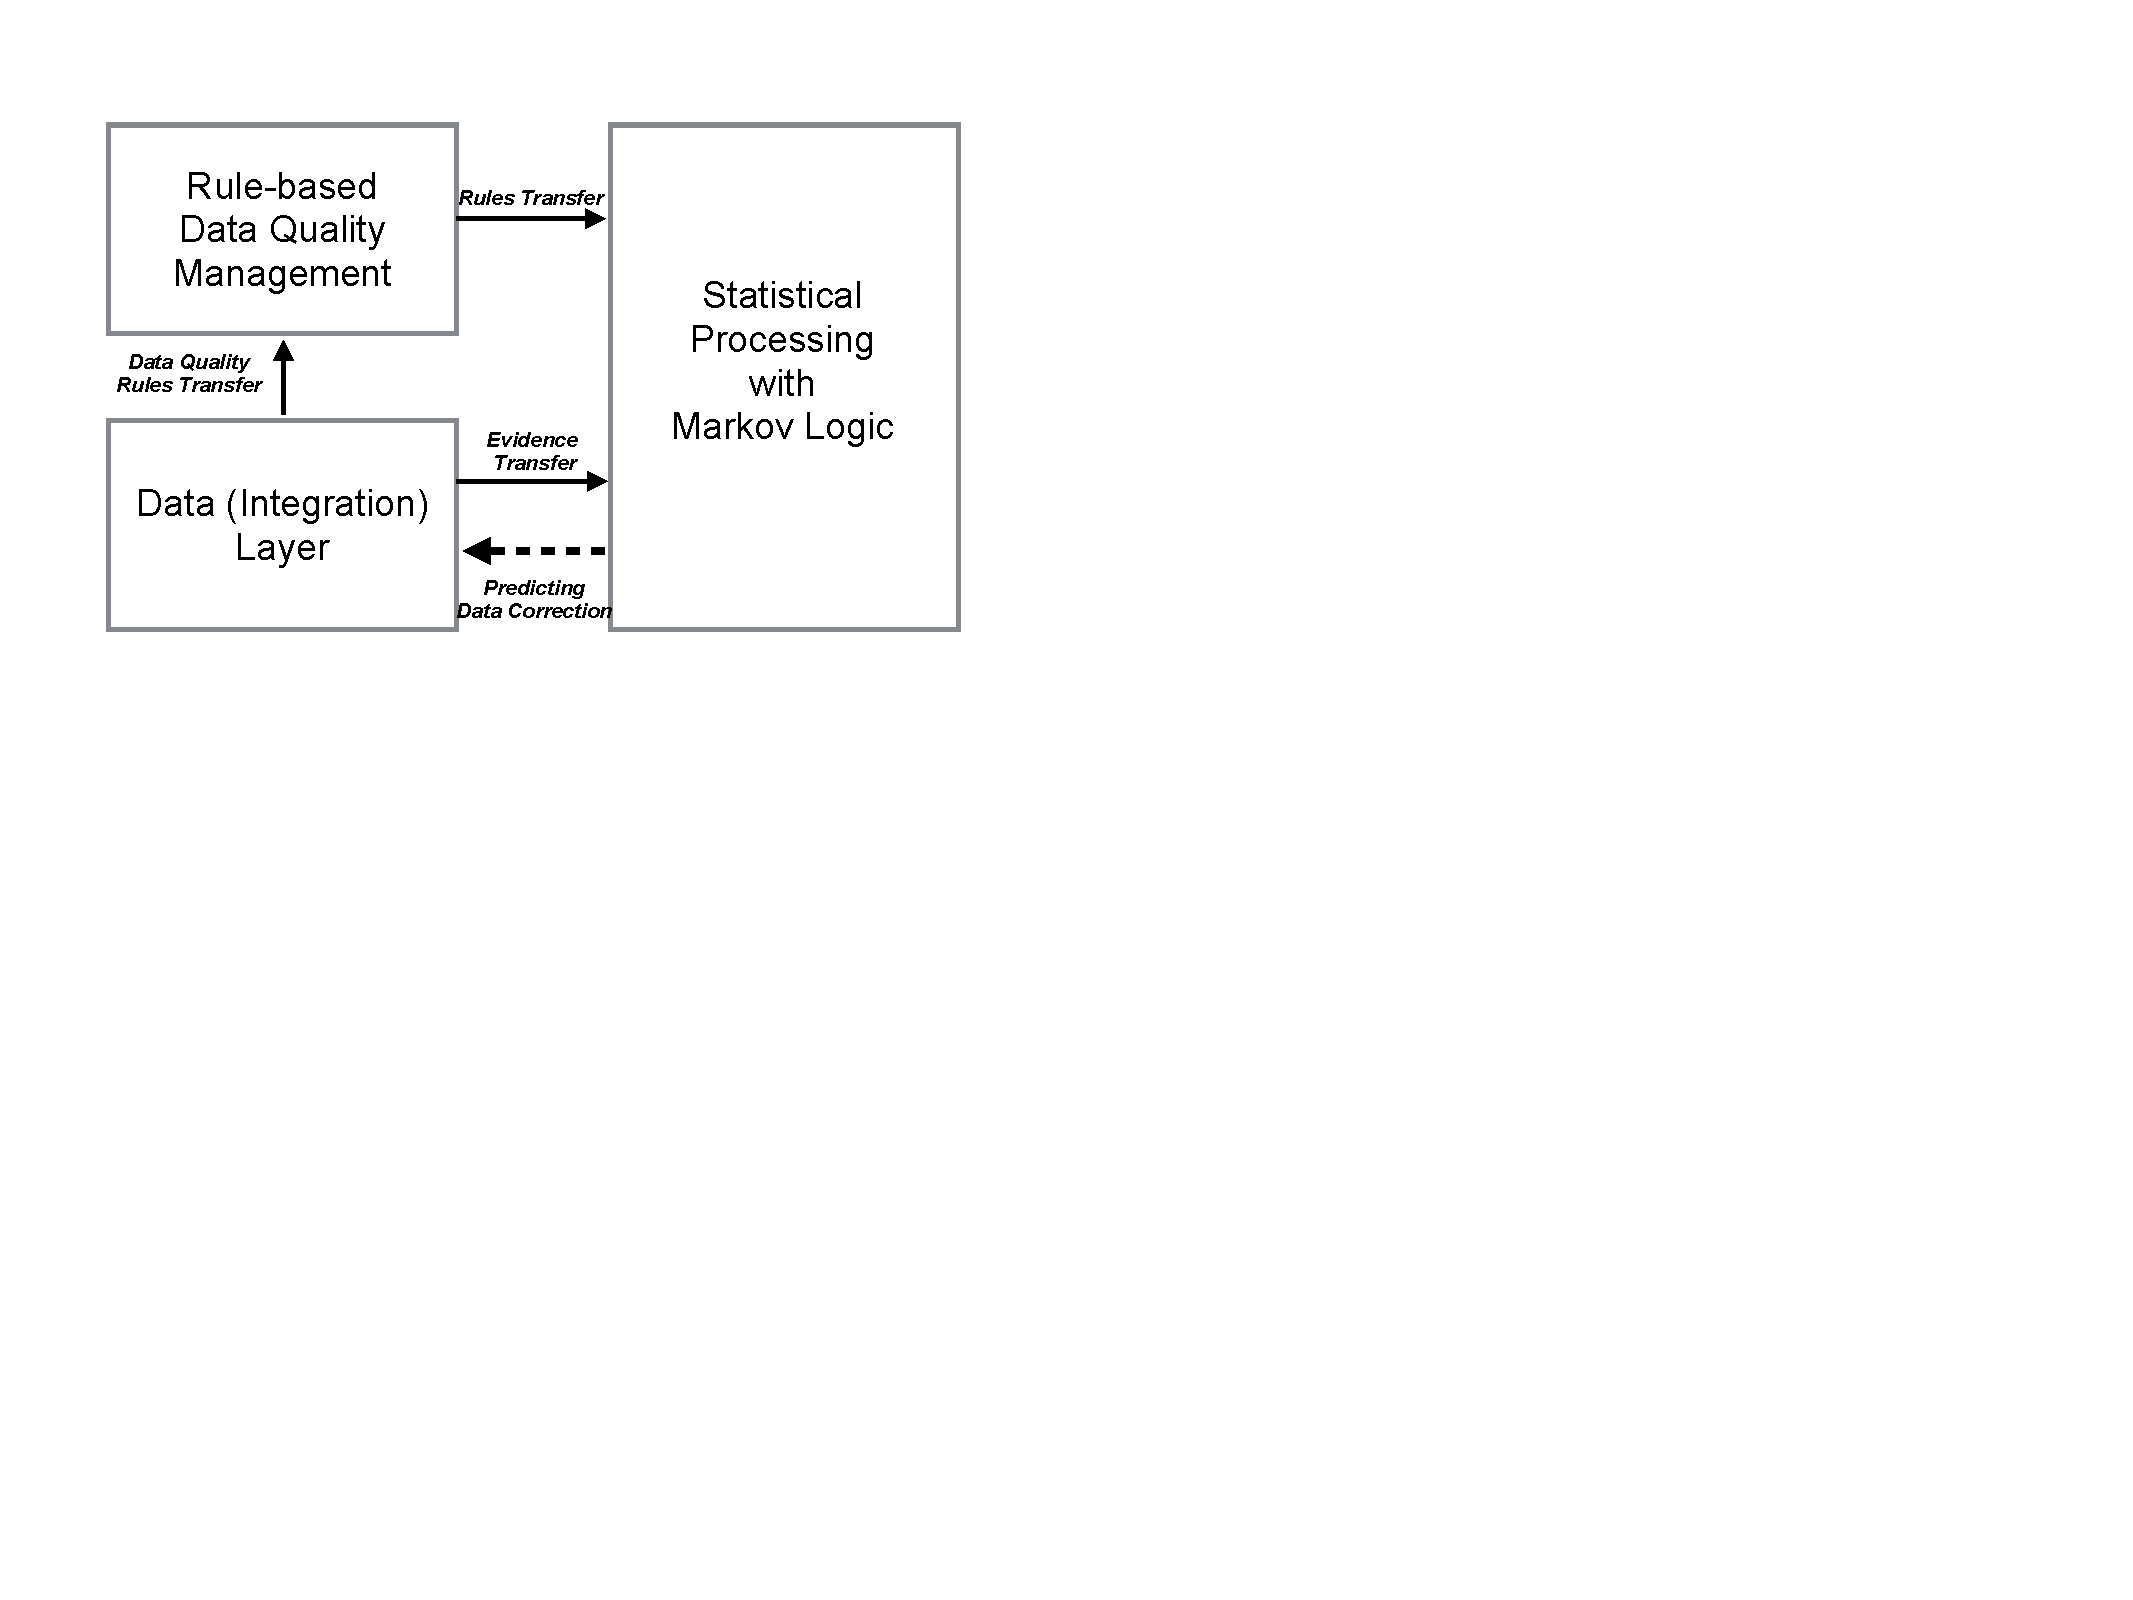
\includegraphics[width=0.9\columnwidth]{img/system.pdf}
 \caption{%\anno{Rmove this picture?} Why? I find this pic useful and supports understanding.
Overview of the proposed data cleaning approach
 %\anno{Please redo this picture to make it look better (e.g., make sure the margins of text to borders are always the same.)} 
 %Our proposed method for data cleaning based on Markov logic consists of three main components: 
 %(I) A \textbf{Rule-based Data Quality Management} component that is based on the data quality rules to address different data quality issues;
 %(II) A \textbf{relation prediction} component based on probabilistic inference performed by the Markov logic framework and (III) 
 %a \textbf{Data Layer} that includes a number of data sources including relational and semi-structured data.}
 %\anno{Figure caption is too long} 
}
 \label{fig:system}
\end{figure}     

We propose to model data cleaning rules in the \textit{Markov logic}~\cite{domingos2009markov} formalism and use probabilistic inference for data cleaning. Markov logic is a knowledge representation system that combines first-order logic as a declarative language and probabilistic graphical models (undirected Markov Networks). On top of this representation we perform probabilistic inference. We introduce technical aspects of Markov logic and joint inference for data cleaning in Section~\ref{subsec:jointinference}.

The main advantage of Markov logic is the ability to reason simultaneously about complex and interacting relationships. By modeling different data cleaning rules as a Markov logic program, we leverage the joint inference on underlying probabilistic graphical model. In this way, we implement \textit{holistic} data cleaning, which is one of main requirements for data cleaning systems \cite{fan2013data, Fan:2014:IRM:2628135.2567657, Dallachiesa:2013:NCD:2463676.2465327}. If no perfect resolution of a rule set is possible, we want to find data cleaning steps that fulfill as many rules as possible while violating only a few~\cite{genesereth1987logical, domingos2009markov}. Therefore, in order to infer the types of errors and their sources, we consider integrity constraints to be probabilistic. We build on an existing approach to specify \textit{soft} functional dependencies between columns~\cite{Ilyas:2004:CAD:1007568.1007641}. 
%Another advantage of Markov Logic is that it allows us to tackle overfitting, a common problem when applying machine learning for repairing errorneous data \anno{You still need to explain overfitting!, EDBT reviewers might not be ML experts}. Overfitting occurs when one applies data quality rules that hold only for a fraction of data, but do not hold globally. Markov logic programs with \textit{"soft"} rules prohibit overfitting by adding weights to the constaint-based rules and incorporating partial knowledge \cite{singla2006entity, poon2008joint, lowd2007recursive}. \note{one more sentence, how does adding weights prohibit overfitting? do we show this experimentally somehow? if not, we might want to remove this paragraph}. 
Moreover, Markov logic enables us to extend traditional data quality rules with semantic constraints~\cite{spies2013knowledge}, meaning that additional knowledge (e.g., in form of predicates that model $\approx$, $\neq,~\leq,\geq$, etc.) is incorporated into conventional data quality rules. This is very helpful in order to capture non-traditional dependencies \cite{chen2009analyses} for data cleaning. %\note{explain this in more detail, I don't understand what you mean}

In the following, we illustrate how to transfer data cleaning rules into Markov logic and leverage probabilistic inference to determine data repair operations for a given data set. See also Figure \ref{fig:system} for high-level overview of our approach. We distinguish between three major components: 
\begin{inparaenum}[\itshape I\upshape)]
\item \textit{Rule-based Data Quality Management} where we specify data-agnostic quality rules to address different data quality issues;
\item \textit{Statistical Inference with Markov Logic} to compute probabilistic data repair based on probabilistic inference performed by the Markov logic framework; and
\item \textit{Data Layer}, which interacts with former two components by providing both integrity constraints and evidence data from a number of data sources including relational and
semi-structured data for Markov logic.
\end{inparaenum}
%\note{YOU NEED TO EXPLAIN FIGURES, NOT JUST REFERENCE THEM *PEITSCH*} *AUTSCH*


\begin{figure*}[t]
 \centering
 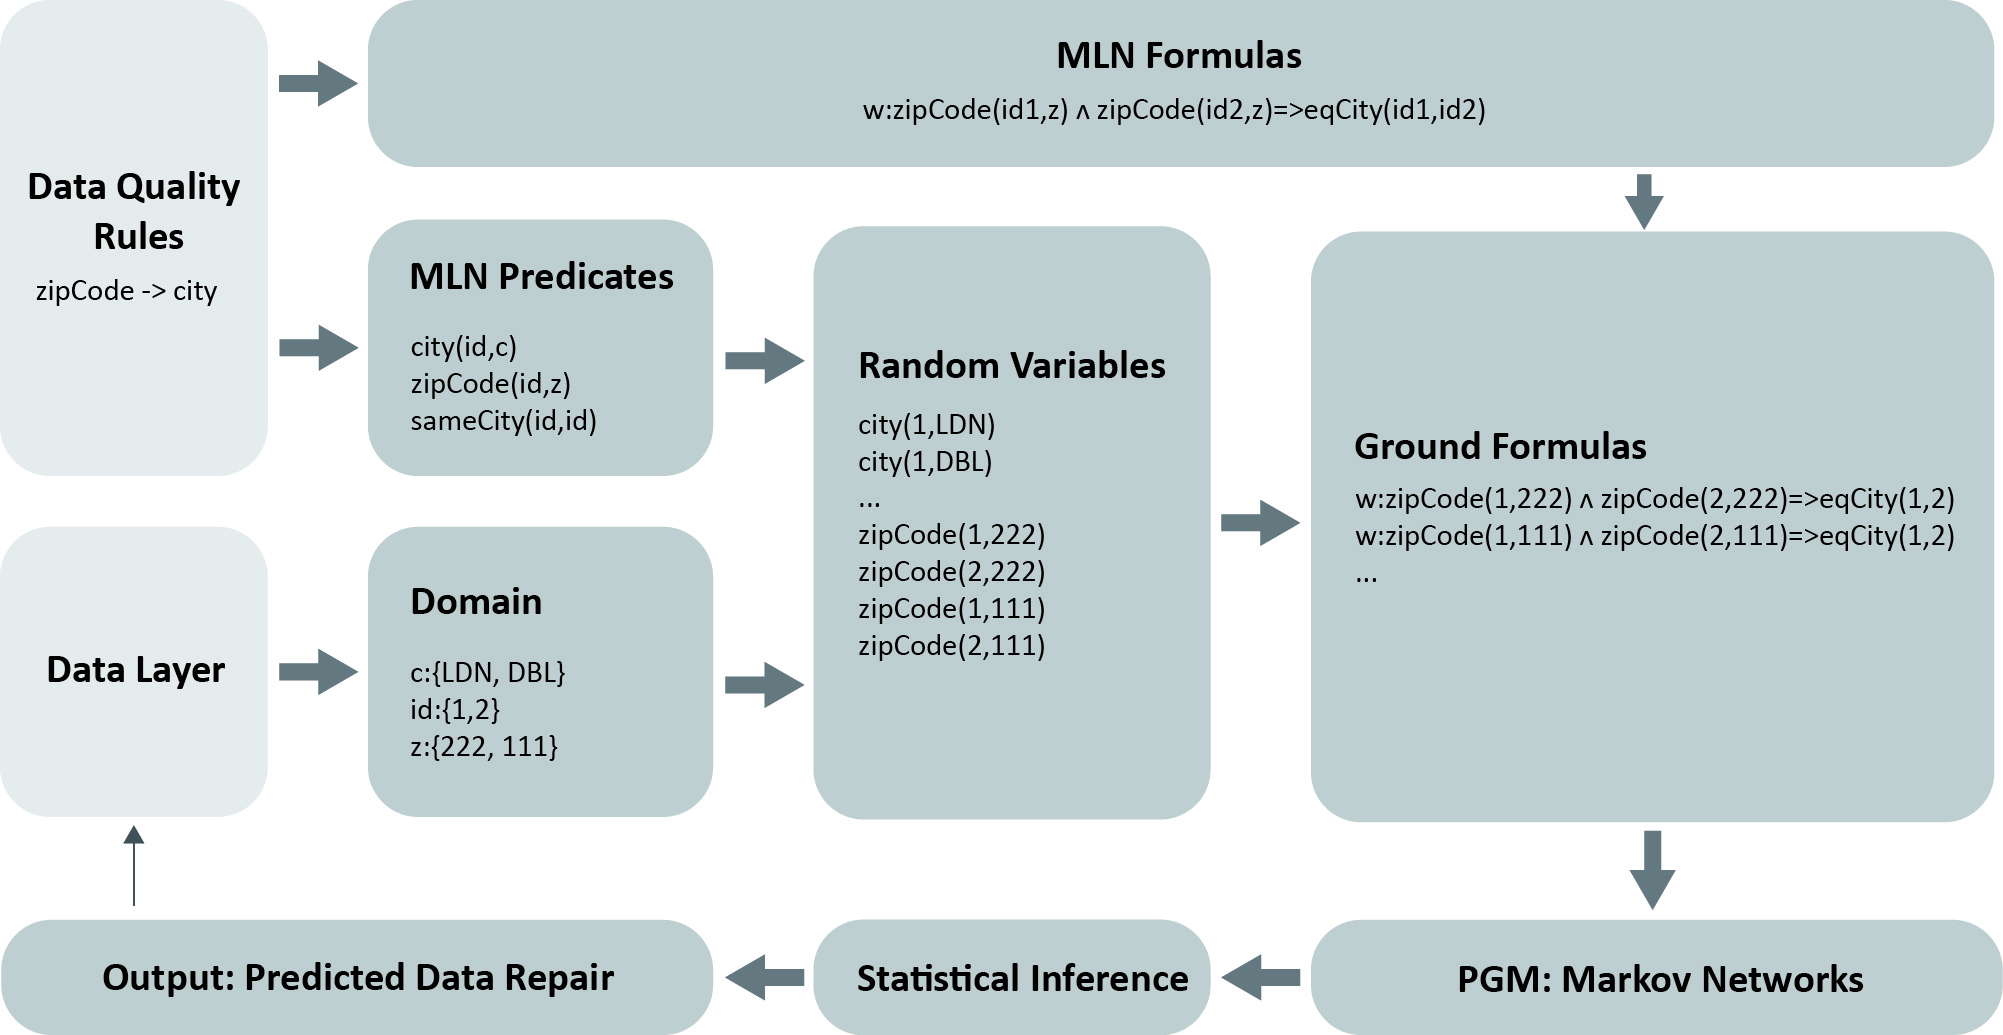
\includegraphics[width=450px, height=200px]{img/mlogic-grounging.jpg}
 \caption{
 %\anno{Please redo this picture to make it look better} this will be really time consuming for now. If I find someone who can do that, I will let them produce sexier picture than this one.
 In context of data cleaning workflow, Markov Logic Network grounding process consists of two phases 
 1) MLN definition by 
(a) fixing MLN schema by defining observed and hidden predicates
(b) domain, which is created from the existing data by considering the MLN schema, and 
(c) specification of weighted first-order logic formulas that represent data cleaning rules;
 2) MLN instantiation by assigning truth values to the all possible instantiations of the MLN predicates by consideration of the domain (Random Variables) and using these ground atoms in formulas. These Ground Formulas constitutes Markov Network in order to compute MAP inference and to estimate the most possible data repair.}
 \label{fig:mlngrounding}
\end{figure*}

\subsection{Compilation of Data Cleaning Rules to \\Predicate Calculus}
\label{sec:ml} 

%\anno{Does your system automate the compilation? If yes, mention this!} - right now, there is a master thesis I am supervising, which implements the automate compilation. 
Next, we describe how to connect the data quality rules formalism to the Markov logic. The base of Markov logic programs is a predicate calculus \cite{genesereth1987logical}, because Markov logic consists of first-order logic sentences. Therefore, we describe a general method to compile formal constraint-based data cleaning rules into predicate calculus. We define data cleaning rules in the form of CFDs and MDs as introduced in Section~\ref{sec:expl}. For example, given the following functional dependency $\phi: X \rightarrow Y$, according to~\cite{Fagin:1982:HCD:322344.322347}, we express $\phi$ as \textit{first-order logic} sentence:
\begin{equation}
\mathsf{\forall x, y_1, y_2, z_1, z_2 \mathcal{R}(x, y_1, z_1) \wedge \mathcal{R}(x, y_2, z_2) \Rightarrow y_1=y_2}
\label{fd2fol}
\end{equation}

In following, we show that first-order logic sentence is crucial for the compilation of data cleaning rules into predictive models. % \note{Aha, why?} - well I think, to understand this, the following explanation is important.
Consider the logical equivalence of the data quality rule $\phi$ in \ref{fd2fol} as a composite component, consisting of subcomponents such as atomic sentences (attribute), logical and quantified sentences (RHS and LHS in FD $\phi$). To describe the structure of $\phi$ in a predicate calculus, we choose symbols that designate the elements of our conceptualization. In connection to the fundamentals of data quality management (c.f.,~Section~\ref{sec:expl}), we define the \textit{vocabulary} we use for the compilation of data quality rules: 
%\anno{WHY ANOTHER VOCABULARY? THIS IS SUPER CONFUSING!!! REWRITE THIS PART TO CONNECT TO THE REST OF THE PAPER}

The \textit{Universe of Disclosure} is specified by the set of all objects from domain $dom(U)$ that is fixed for the set of attributes $attr(\mathcal{R})$. A \textit{term} is used as a name for an object in the universe of discourse. We define \textit{variables} to denote arguments in atoms and \textit{constants} to denote data constants of particular domain $dom(U_i)$ of an $i$-th attribute $U_i \in attr(\mathcal{R})$. To designate the tuple in relation $\mathcal{R}$: $\mathcal{R}(x_1,x_2, \dots , x_n)$, we use atomic sentences $\mathsf{\textsl{attr-X}_1(id,v_1)}$, $\mathsf{\textsl{attr-X}_2(id,v_2)}$ $\dots$ $\mathsf{\textsl{attr-X}_n(id,v_n)}$ where $\mathsf{\textsl{attr-X}_i(id,v_i)}$ means that $\mathsf{v_i}$ is a attribute value of the $i$-th attribute in $\mathcal{R}(x_1,x_2, \dots , x_n)$ of the $id$-th tuple in relation $\mathcal{R}$. \textit{Relation constants} denote relations between several objects:
	\begin{itemize}
		\item Similarity: $\mathsf{\textsl{similar}(x_1,x_2)}$ means that $\mathsf{x_1}$ similar to $\mathsf{x_2}$ (e.g., by using different similarity measures like cosine or Jaccard similarities).
		\item Equality: $\mathsf{\textsl{equal-X}(id_1, id_2)}$ means that the values of the attribute X of two tuples $\mathsf{id_1}$ and $\mathsf{id_2}$ should be equal.
		\item Matching: $\mathsf{\textsl{match-X}(id_1, id_2)}$ means that values of two tuples $\mathsf{id_1}$ and $\mathsf{id_2}$ of the attribute X are identified to match.
		\item Custom Predicate: used for encoding diverse semantic constraints (e.g. \textit{contains}, \textit{between}, \textit{less} etc.), which are not part of the data constraints.
	\end{itemize}

%\note{Is the compilation more than a slightly different syntax? What are the challenges? This is one of the contributions, need more elaboration.} this is formalization, previous reviewer has asked for.
Given this vocabulary, we describe our conceptualization of the data quality rules with predicate-calculus sentences. For example, for the functional dependency $\phi: X \rightarrow Y$ and the first-order logic sentence in Formula \ref{fd2fol}, we compile to the corresponding Markov logic formula as follows:
\begin{flalign*}
  & \mathsf{\textsl{attr-X}(id_1, x) \wedge \textsl{attr-X}(id_2, x) \Rightarrow \textsl{equal-Y}(id_1, id_2)} & 
\end{flalign*}
\vspace*{-0.5cm}

Analogously, we translate a matching dependency $ \mu: \mathcal{S}_1[x_1]\approx \mathcal{S}_2[x_2]\rightarrow \mathcal{S}_1[y_1]\rightleftharpoons \mathcal{S}_2[y_2]$ on a database instance $\mathcal{D}$ with two relational schemas $\mathcal{S}_1$ and $\mathcal{S}_2$ as follows:
\begin{flalign*}
  & \mathsf{\textsl{attr-X/S1}(id_1, x_1) \wedge \textsl{attr-X/S2}(id_2, x_2) \wedge \textsl{similar}(x_1, x_2)} & \\
  & \mathsf{\Rightarrow \textsl{S1/match-Y/S2}(id_1, id_2)} & 
\end{flalign*}
\vspace*{-0.5cm}

If we specify a matching dependency using two relations, we need to mark the attributes corresponding to a relation with that relation $\mathsf{\textsl{attr-X/}}\mathcal{R}$. Furthermore, as introduced above, we use predicates to represent operators in the data quality as shown in Table \ref{tab:concept}.

\begin{table}[h]\footnotesize
%\scriptsize
\centering
\begin{tabular}{@{}lcl@{}}
\toprule
Concept    & Operator & Predicate \\ \midrule
Similarity & $\mathcal{S}_1[x_1]\approx \mathcal{S}_2[x_2]$        & $\mathsf{\textsl{similar}(x_1,x_2)}$ \\
Equality   & $y_1=y_2$ & $\mathsf{\textsl{equal-Y}(id_1, id_2)}$ \\
Matching   & $\mathcal{S}_1[y_1]\rightleftharpoons \mathcal{S}_2[y_2]$   & $\mathsf{\textsl{S1/match-Y/S2}(id_1, id_2)}$ \\ \bottomrule
\end{tabular}
\caption{Markov logic predicates used for data cleaning.}
\label{tab:concept}
\end{table}

%\anno{TOO GENERIC AND HIGH LEVEL, SOUNDS LIKE A COPY FROM AN ML TEXTBOOK. CONNECT THIS TO OUR PROBLEM! -> this is not a copy from any books.
% but you are correct, this should be connected to the backend of the method.
%MLNs are created by writing a set of first-order logic rules with weights, constructed using variables that range of objects in the domain of interest and predicates that represent relations between these objects. Predicates can be observed or hidden. \textit{Observed predicates} are relations between objects that can be seen in a given data set. $\mathsf{\textsl{attr-X}_1(id,v_1)}$, $\mathsf{\textsl{attr-X}_2(id,v_2)}$ $\dots$ $\mathsf{\textsl{attr-X}_n(id,v_n)}$  where $\mathsf{\textsl{attr-X}_i(id,v_i)}$ are observed predicates. In addition, an MLN may have a number of \textit{hidden predicates}, meaning that they are not observed in the input data, but can be inferred through rules. In our case, $\mathsf{\textsl{equal-Y}(id_1, id_2)}$ and $\mathsf{\textsl{S1/match-Y/S2}(id_1, id_2)}$ are hidden.  The goal of probabilistic inference is to infer the likelihood for observed and hidden predicates given a rule set and evidence. We define the MLN in such a way that reasoning about hidden predicates given evidence and data cleaning rules allows us to determine data repair operations.}

%\subsubsection{First-Order Logic Formulae}
%\note{Explain why we are doing all of this? What is the advantage?} 
We assume that integrity constraints have been already determined by using methods reviewed in \cite{liu2012discover} or specified by domain experts manually. To demonstrate the compilation of the data cleaning rules into Markov logic, have a look at the CFD from the motivation example in Section~\ref{sec:expl}. This CFD states that if any two tuples agree on attribute values for $\mathsf{\textsl{city}}$ and $\mathsf{\textsl{phone}}$, then the attribute values on $\mathsf{\textsl{street}}$ and $\mathsf{\textsl{zip}}$ should agree as well:
\begin{equation*}
\mathsf{fd: \textsc{transaction}([\textsl{city}, \textsl{phone}] \rightarrow [\textsl{street}, \textsl{zipcode}])}
\end{equation*}
\vspace*{-0.5cm}

To enable straightforward compilation, we assume that CFDs are provided in normal form. This means if $\psi(X \rightarrow Y_1,Y_2,\dots , T_p)$, then $\psi$ will be decomposed into several CFDs where $RHS(\psi)$ (right hand side of $\psi$) becomes a single attribute: $\psi_1(X \rightarrow Y_1 , T_p)$, $\psi_2(X \rightarrow Y_2 , T_p) \dots$. Following the normalization rule for functional dependencies, we split the $\mathsf{fd}$ rule into two rules:
\begin{flalign*}
& \mathsf{cfd_1: \textsc{transaction}([\textsl{city}, \textsl{phone}] \rightarrow [\textsl{street}], t_1=(\_, \_ \parallel  \_))}& \\
& \mathsf{cfd_2: \textsc{transaction}([\textsl{city}, \textsl{phone}] \rightarrow [\textsl{zipcode}], t_2=(\_, \_ \parallel  \_))}&
\end{flalign*}
\vspace*{-0.5cm}

According to~\cite{Fagin:1982:HCD:322344.322347} we represent these $\mathsf{cfd_1}$ and $\mathsf{cfd_2}$ as two first-order logic formulas:
\begin{flalign*}
& \mathsf{1)~\forall~\textsl{city}, \textsl{phone}, \textsl{street}_1, \textsl{street}_2 }& \\
& \mathsf{\textsc{transaction}(\textsl{city}, \textsl{phone}, \textsl{street}_1)~\wedge}&\\
& \mathsf{\textsc{transaction}(\textsl{city}, \textsl{phone}, \textsl{street}_2) }& \\
& \mathsf{ \Rightarrow \textsl{street}_1=\textsl{street}_2 }& \\
& \mathsf{2) ~\forall~\textsl{city}, \textsl{phone}, \textsl{zip}_1, \textsl{zip}_2 }& \\
& \mathsf{ ~\textsc{transaction}(\textsl{city}, \textsl{phone}, \textsl{zip}_1) \wedge}& \\
& \mathsf{\textsc{transaction}(\textsl{city}, \textsl{phone}, \textsl{zip}_2) }& \\
& \mathsf{ \Rightarrow \textsl{zip}_1=\textsl{zip}_2 }&
\end{flalign*}
\vspace*{-0.3cm}

These formulas state that if two tuples of the \textsc{transaction} relation agree on the \textsl{city} and \textsl{phone} values, then their \textsl{street} and \textsl{zip} values should be the same. Once we have formulated our integrity constraints as first-order logic formulas, we translate them into Markov
logic syntax. We illustrate this with the first-order logic formulas $\mathsf{1)}$ and $\mathsf{2)}$ as defined above.
Given that every attribute from the schema $\mathsf{\textsc{transaction}}$ is expressed as a predicate, we need two predicates, 
namely $\mathsf{\textsl{city}(id, city)}$ and $\mathsf{\textsl{phone}(id, phone)}$ to encode the LHS of $\mathsf{fd}$. They indicate the values for the fields \textsl{city} and \textsl{phone} for each tuple. The full example is given in Table~\ref{tab:mlndeclare}, which shows all steps in predicate translation and how data from our example database is translated into grounded atoms. Additionally, we define two predicates for our data quality rule, namely $\mathsf{\textsl{equal-street}(id, id)}$ and $\mathsf{\textsl{equal-zip}(id, id)}$. These predicates model equality of two values of the attribute \textsl{street} respectively \textsl{zip} (as denoted by the $\mathsf{fd}$ rule above):

\begin{flalign*}
	& \mathsf{1)  \textsl{city}(id_1, city) \wedge \textsl{city}(id_2, city) \wedge \textsl{phone}(id_1, phone) }& \\ 
	& \mathsf{  \wedge \textsl{phone}(id_2, phone) \Rightarrow \textsl{equal-street}(id_1, id_2)} & \\
	& \mathsf{2)  \textsl{city}(id_1, city) \wedge \textsl{city}(id_2, city) \wedge \textsl{phone}(id_1, phone) }& \\ 
	& \mathsf{  \wedge \textsl{phone}(id_2, phone) \Rightarrow \textsl{equal-zip}(id_1, id_2)} & 
\end{flalign*}
\vspace*{-0.5cm}

Note that using the same arguments in predicates $\mathsf{\textsl{city}(id, city)}$ and $\mathsf{\textsl{phone}(id, phone)}$ encodes equality of the corresponding values in the Markov logic program. The two different tuples are distinguished by $\mathsf{id_1}$ and $\mathsf{id_2}$. 
These data quality rules form the basis for a Markov logic program. A particular advantage of Markov logic is its \textit{modularity} while modeling. We create "complex" statistical models by combining various "atomic" models. Thereby, we consider each declared data quality rule as an "atomic" probabilistic model. In combination, these small models form a "compound" model. So far we have shown how to express integrity constraints in terms of the predicate calculus.
Having declared the data quality rules by capturing all correlations and constraints, we now infer potential predicates, such as $\mathsf{\textsl{equal-street}(id, id)}$. This predicate holds the information about possible repairs on the attribute $\mathsf{\textsl{street}}$ in the \textsc{transactions} tables in our running example from Section~\ref{sec:expl}. Reasoning about such hidden predicates allows us to decide which attributes gets a particular repair. 

\begin{table}[t]\footnotesize
\scriptsize
\centering
\resizebox{\columnwidth}{!}{%
\begin{tabular}{@{}ll@{}}
\toprule
Phase                                                                             & Example                                                                                                                                                          \\ \midrule
1) Schema definition                                                              & \begin{tabular}[c]{@{}l@{}}$t_2$(item, firstname, lastname, street,\\ city, zipcode, phone)\end{tabular}                                                              \\ \midrule
\begin{tabular}[c]{@{}l@{}}2) Observed predicates \\ MLN declaration\end{tabular} & \begin{tabular}[c]{@{}l@{}}$\mathsf{\textsl{firstname}(id, value)}$ \\ $\mathsf{\textsl{lastname}(id, lastname)}$ \\ $\mathsf{\textsl{street}(id, street)}$ \\ $\mathsf{\textsl{city}(id, city)}$\\ $\mathsf{\textsl{zip}(id, code)}$ \\ $\mathsf{\textsl{phone}(id, num)}$\end{tabular} \\ \midrule
3) Data                                                                           & \begin{tabular}[c]{@{}l@{}}$t_2$(Galaxy 5, NULL, Miller, \\ 12 Hay St., NULL, 818, 11234)\end{tabular}                                                              \\ \midrule
4) Grounded (evidence) atoms                                                      & \begin{tabular}[c]{@{}l@{}} $\mathsf{\textsl{item}(2, Galaxy5)}$ \\ $\mathsf{\textsl{lastname}(2, Miller)}$ \\ $\mathsf{\textsl{street}(2, 12HaySt.)}$ \\ $\mathsf{\textsl{zip}(2, 818)}$ \\ $\mathsf{\textsl{phone}(2, 11234)}$\end{tabular}                         \\ \bottomrule
\end{tabular}}
\caption{\label{tab:mlndeclare} MLN declaration process and creation of grounded atoms for Tuple 2 in the \textsc{Transactions} example table.}
\end{table}
\subsection{Data Repair as Joint Inference}
\label{subsec:jointinference}
Markov logic defines a knowledge representation system that combines first-order logic as a declarative language with probabilistic graphical models (undirected Markov Networks MLNs) on top of which we perform probabilistic inference. Semantically, a MLN is a log-linear model, which defines the probability distribution over possible worlds, in our case all possible states in the database.

We create MLNs by writing a set of first-order logic rules (c.f., Section~\ref{sec:ml}) with weights by using predicates that represent relations between these objects. We distinguish between observed and hidden predicates. \textit{Observed predicates} are relations between objects which exist in a given dataset: $\mathsf{\textsl{attr-X}_1(id,v_1)}$, $\mathsf{\textsl{attr-X}_2(id,v_2)}$ $\dots$ $\mathsf{\textsl{attr-X}_n(id,v_n)}$ are observed predicates, which encode that $\mathsf{\textsl{attr-X}_i}$ has value $\mathsf{v_i}$ on tuple $\mathsf{id}$. In addition, an MLN may have a number of \textit{hidden predicates}, which are not present in the input data, but may be inferred through rules. In our case, $\mathsf{\textsl{equal-Y}(id_1, id_2)}$ and $\mathsf{\textsl{S1/match-Y/S2}(id_1, id_2)}$ are hidden.  The goal of probabilistic inference is to infer the likelihood for observed and hidden predicates given a rule set and evidence. We define the MLN in such a way that reasoning about hidden predicates given evidence and data cleaning rules allow us to determine data repair operations. In other words, we perform an inference task as a prediction for the data cleaning.
We create MLNs by writing a set of first-order logic rules (c.f., Section~\ref{sec:ml}) with weights by using predicates that represent relations between these objects. We distinguish between observed and hidden predicates. \textit{Observed predicates} are relations between objects which exist in a given dataset: $\mathsf{\textsl{attr-X}_1(id,v_1)}$, $\mathsf{\textsl{attr-X}_2(id,v_2)}$ $\dots$ $\mathsf{\textsl{attr-X}_n(id,v_n)}$ are observed predicates, which encode that $\mathsf{\textsl{attr-X}_i}$ has value $\mathsf{v_i}$ on tuple $\mathsf{id}$. In addition, an MLN may have a number of \textit{hidden predicates}, which are not present in the input data, but inferred through rules. In our case, $\mathsf{\textsl{equal-Y}(id_1, id_2)}$ and $\mathsf{\textsl{S1/match-Y/S2}(id_1, id_2)}$ are hidden.  The goal of probabilistic inference is to infer the likelihood for observed and hidden predicates given a rule set and evidence. We define the MLN in such a way that reasoning about hidden predicates given evidence and data cleaning rules allow us to determine data repair operations. In other words, we perform an inference task as a prediction for the data cleaning.

%%%%%%
An important step in our method is the \textit{grounding} of the MLN (in details illustrated in Figure \ref{fig:mlngrounding}). 
%\note{EXPLAIN THIS FIGURE IN DETAIL *PEITSCH*} - ok, but there is a lot of explanation here, and if we put everything here, then this will disturb the reading flow. Would it be acceptable to provide details in figure caption?! 
Because constraint-based rules are data agnostic~\cite{fan2012foundations}, we need to ``ground'' previously defined predicates with the available evidence, in our case the database to process. We take the content of the database (a set of tuples) and produce a set of observed predicates (so-called \textit{grounded atoms}). Let $n$ denote the number of schema attributes. Then we convert each tuple from the database into $n$ different Markov logic evidence atoms. For example, we translate transaction 2 in our running example into the following 6 grounded atoms: \textsl{item}(2, Galaxy 5), \textsl{firstname}(2, Max), \textsl{lastname}(2, Miller), \textsl{street}(2, 12 Hay St.), \textsl{zip}(2, 818) and \textsl{phone}(11234). These are examples of observed predicates for the dataset. Table~\ref{tab:mlndeclare} summarizes the process of the groundings creation. We use these groundings (or evidence atoms) in the joint inference for data cleaning. 
%%%%%
Given an MLN that models data cleaning rules, let $q \in \mathcal{L}^n$ denote a hidden predicate with $n$ \emph{literals} (random variables) $L_1,...,L_n$, where each literal $L_i$
has $2$ discrete states, $L_i = \lbrace 0,1 \rbrace$.
Then, the MLN is a joint distribution on  $L_1,...,L_n$ that 
is specified by a vector $\phi(q)$ of $d$ integer values, where
each element represents the number of true groundings of the 
corresponding literal in the formula and $d$ denotes the 
maximum number of literals in a given formula. Additionally, 
we have a weight/parameter vector $\theta \in \mathcal{R}^d$:
%\vspace{-3em}
\begin{equation*}
Pr \left( q | \theta \right) = 
\frac{1}{Z(\theta)} \exp\left( \langle \theta, \phi(q) \rangle  \right), 
Z(\theta) = \sum_{q \in \mathcal{L}^n}\exp\left( \langle \theta, \phi(q) \rangle  \right) 
\end{equation*}
%\vspace{-2em}
where $\langle \theta, \phi(q) \rangle$ denotes a dot product. 
$Z(\theta)$ is the normalization constant also called the 
\emph{partition function}. Since the partition function is a constant and the exponential is monotonic, finding the MAP assignment in our data cleaning problem is equivalent to finding the assignment $q_M$ that maximizes the probability $Pr \left( q | \theta \right)$.

The output of the inference are data repair operations; e.g., the hidden predicate \textsl{equal-street} may be determined to have (among other groundings) the following likely value: $\mathsf{\textsl{equal-street}(1, 3)}$, indicating that the \textsl{street} field for transaction 3 should have the same value as the \textsl{street} field of transaction 1. In this case, the data repair operation is to replace the \textsc{null} value in transaction 3 with the address ``1 Sun Dr.''. 
%\note{Shouldn't the MLN allow us to inspect the uncertainty in these decisions? Can you elaborate on that?}  I was thinking about this. Because we are using MAP, we assume that we take the most possible solution. otherwise we would need to explain all of the Markov logic + Markov networks here.
As we noted in the discussion of the running example, there is an interplay of different rules that affects the probability of hidden predicates. Therefore, the inference produces the most likely state of the entire Markov Logic Network with regards to all integrity constraints. The probabilities for the hidden predicates are therefore influenced by \textit{all} defined data quality rules. By running the inference over the entire database, we predict the most likely data repairs for our data set by determining the most likely grounding of the hidden predicates and this reduces to computing \textsc{map} inference on the MLN model.      

The difficulty in designing algorithms for MAP inference arises when finding an efficient way to reason about the large number of possible assignments to the variables in the model. In terms of theoretical guarantees, inference is NP-hard or or computationally intractable and as proven by \cite{Shimony1994} in many cases cannot be approximated. Amongst the numerous techniques that are available to solve MAP inference problems, we chose to cast the inference problem as an \emph{integer linear program} (ILP)\cite{Sontag10approximateinference}. Another competitive approach called \emph{message passing} perform \emph{belief propagation} along the edges of the graphical model. Although, message passing is straightforward to implement it has troubles converging \cite{schwing2011distributed, felzenszwalb2006efficient, pritch2009shift} and tends not to give as good results as ILP~\cite{NoessnerNS13}. 



%%%%%%%%%%%%%%%%%%%%%%%%%%%%%%%%%%%%%%%%%%%%%%%%%%%%%%%%%%%%%%%%%%%%%%%%
% Evaluation
%%%%%%%%%%%%%%%%%%%%%%%%%%%%%%%%%%%%%%%%%%%%%%%%%%%%%%%%%%%%%%%%%%%%%%%%
\section{Experimental Study}
\label{sec:evaluation}

%-------plots------
\begin{table*}[!htbp]\footnotesize
\scriptsize
\begin{tabular}{lll}

%HOSP 
\begin{tikzpicture}
    \begin{axis}[
        legend pos=outer north east,        
        title=(a) \textsc{hosp} Data Cleaning for 90k,
        xlabel=noise,
        ylabel=F1, ]

         \addplot[mark=diamond] table[x=NOISE, y=CFDF1] {data/hosp-evaluation-90-datasize.tsv};
         \addplot table[x=NOISE, y=MDF1] {data/hosp-evaluation-90-datasize.tsv};
         \addplot table[x=NOISE, y=CFDMDF1] {data/hosp-evaluation-90-datasize.tsv};

        \legend{$cfd$,$md$,$cfd+md$},

    \end{axis}
\end{tikzpicture}
    &  
    

    \begin{tikzpicture}
%\selectcolormodel{gray}
   \begin{axis}[
       legend pos=outer north east,
       title=(b) \textsc{hosp} Data Cleaning for noise 10\%,
       xlabel=data size in k,
       ylabel=F1, ]

         \addplot[mark=diamond] table[x=DATASIZE, y=CFDF1] {data/hosp-evaluation-10-noise.tsv};
         \addplot table[x=DATASIZE, y=MDF1] {data/hosp-evaluation-10-noise.tsv};
         \addplot table[x=DATASIZE, y=CFDMDF1] {data/hosp-evaluation-10-noise.tsv};

       \legend{$cfd$,$md$,$cfd+md$},

   \end{axis}
\end{tikzpicture}
&
\begin{tikzpicture}
%\selectcolormodel{gray}
   \begin{axis}[
       legend pos=outer north east,
       title=(c) Runtime for \textsc{hosp} Data Cleaning,
       xlabel=data size in k,
       ylabel=seconds, ]

         \addplot[mark=diamond] table[x=DATASIZE, y=TIME] {data/hosp-evaluation-2-noise.tsv};
         \addplot table[x=DATASIZE, y=TIME] {data/hosp-evaluation-4-noise.tsv};
         \addplot table[x=DATASIZE, y=TIME] {data/hosp-evaluation-6-noise.tsv};
         \addplot table[x=DATASIZE, y=TIME] {data/hosp-evaluation-8-noise.tsv};
         \addplot table[x=DATASIZE, y=TIME] {data/hosp-evaluation-10-noise.tsv};

       \legend{$noise 2$,$noise 4$,$noise 6$,$noise 8$,$noise 10$},

   \end{axis} 
   \end{tikzpicture}

 \\
%TPC-H results

\begin{tikzpicture}
%\selectcolormodel{gray}
  \begin{axis}[
      legend pos=outer north east,
      title=(d) \textsc{tpc-h} Data Cleaning for 20k,
      xlabel=noise,
      ylabel=F1, ]

         \addplot[mark=diamond] table[x=NOISE, y=CFDF1] {data/tpch-evaluation-20000-datasize.tsv};
         \addplot table[x=NOISE, y=MDF1] {data/tpch-evaluation-20000-datasize.tsv};
         \addplot table[x=NOISE, y=CFDMDF1] {data/tpch-evaluation-20000-datasize.tsv};

      \legend{$cfd$,$md$,$cfd+md$},

  \end{axis}
\end{tikzpicture}

& \begin{tikzpicture}
%\selectcolormodel{gray}
  \begin{axis}[
      legend pos=outer north east,
      title=(e) \textsc{tpc-h} Data Cleaning for noise 2\%,
      xlabel=data size,
      ylabel=F1, ]

         \addplot[mark=diamond] table[x=DATASIZE, y=CFDF1] {data/tpch-evaluation-2-noise.tsv};
         \addplot table[x=DATASIZE, y=MDF1] {data/tpch-evaluation-2-noise.tsv};
         \addplot table[x=DATASIZE, y=CFDMDF1] {data/tpch-evaluation-2-noise.tsv};

      \legend{$cfd$,$md$,$cfd+md$},

  \end{axis}
\end{tikzpicture} & 

\begin{tikzpicture}
%\selectcolormodel{gray}
  \begin{axis}[
      legend pos=outer north east,
      title=(f) Runtime for TPCH Data Cleaning,
      xlabel=data size,
      ylabel=seconds, ]

         \addplot[mark=diamond] table[x=DATASIZE, y=TIME] {data/tpch-evaluation-2-noise.tsv};
         \addplot table[x=DATASIZE, y=TIME] {data/tpch-evaluation-4-noise.tsv};
         \addplot table[x=DATASIZE, y=TIME] {data/tpch-evaluation-6-noise.tsv};
         \addplot table[x=DATASIZE, y=TIME] {data/tpch-evaluation-8-noise.tsv};
         \addplot table[x=DATASIZE, y=TIME] {data/tpch-evaluation-10-noise.tsv};

      \legend{$noise 2$,$noise 4$,$noise 6$,$noise 8$,$noise 10$},

  \end{axis}
\end{tikzpicture}
\end{tabular}
\caption{\label{tab:plots} \anno{Y-SCALE OF d and e is broken!!!} Evaluation of the data repair method based on Markov logic applied on the ~\textsc{hosp} and~\textsc{tpc-h} data sets. (a)-(c) Data repair on \textsc{hosp} with an extended Markov logic method. (d)-(f) Experimental study of the Markov logic data cleaning on synthetic data set \textsc{tpc-h}.}
\end{table*}


\begin{table}[t]\footnotesize
%\scriptsize
\centering
\begin{tabular}{@{}cccc@{}}
\toprule
{\bf dataset}       & 
{\bf \begin{tabular}[c]{@{}c@{}}numer \\ of tuples\end{tabular}} & 
{\bf \begin{tabular}[c]{@{}c@{}}number\\ of formulas\end{tabular}}  & 
{\bf \begin{tabular}[c]{@{}c@{}}runtime\\ (sec)\end{tabular}} \\ 
                                                         \\
\midrule
                     & 63K                                                                                                                     & 21                                                                                                                                        & 242                                                           \\
{\bf \textsc{hosp}}           & 83K                                                                                                                      & 21                                                                                                                                        & 477                                                           \\
\multicolumn{1}{l}{} & 143K                                                                                                                    & 21                                                                                                                                        & 1107                                                          \\ \midrule
\multicolumn{1}{l}{} & 20K                                                                                                                      & 15                                                                                                                                        & 41                                                            \\
{\bf \textsc{tpc-h}}           & 40K                                                                                                                      & 15                                                                                                                                        & 131                                                           \\
\multicolumn{1}{l}{} & 100K                                                                                                                     & 15                                                                                                                                        & 732                                                           \\ \bottomrule
\end{tabular}
\caption{\label{tab:runtime} Scalability of the data cleaning for \textsc{tpc-h} and \textsc{hosp} data sets (with fixed noise 4\%). }
\end{table}


\begin{table*}[t]\footnotesize
\scriptsize
\centering
\begin{tabular}{@{}llll@{}}
\toprule
& \multicolumn{1}{c}{\textsc{hosp}}  & \multicolumn{1}{c}{\textsc{tpc-h}}  & \multicolumn{1}{c}{\textsc{msag}}  \\ \midrule
\begin{tabular}[c]{@{}l@{}}
 observed\\ predicates
\end{tabular} 
& 
\begin{tabular}[c]{@{}l@{}}
\textsl{providerNr/\textsc{hosp}}(hid, pn)\\ 
\textsl{hospitalName/\textsc{hosp}}(hid, n)\\ 
\textsl{address/\textsc{hosp}}(hid, add)\\ 
\textsl{city/\textsc{hosp}}(hid, c)\\ 
\textsl{state/\textsc{hosp}}(hid, st)\\ 
\textsl{zipCode/\textsc{hosp}}(hid, code)\\ 
\textsl{countryName/\textsc{hosp}}(hid, country)\\ 
\textsl{phoneNumber/\textsc{hosp}}(hid, numb)\\ 
\textsl{condition/\textsc{hosp}}(hid, cond)\\ 
\textsl{measureCode/\textsc{hosp}}(hid, mcode)\\ 
\textsl{measureName/\textsc{hosp}}(hid, mname)\\ 
\textsl{score/\textsc{hosp}}(hid, score)\\ 
\textsl{zip/\textsc{zipcode}}(zid, code)\\ 
\textsl{state/\textsc{zipcode}}(zid, st)
\end{tabular}                       
& 
\begin{tabular}[c]{@{}l@{}}
\textsl{custKey}(id, key)\\ 
\textsl{name}(id, n)\\ 
\textsl{addr}(id, add)\\ 
\textsl{natKey}(id, nkey)\\ 
\textsl{phone}(id, ph)\\ 
\textsl{acc}(id, a)\\ 
\textsl{mrkt}(id, m)\\ 
\textsl{orderKey}(id, okey)\\ 
\textsl{orderStatus}(id, st)\\ 
\textsl{totalPrice}(id, p)\\ 
\textsl{orderDate}(id, d)\\ 
\textsl{orderPriority}(id, pr) \\ 
\textsl{clerk}(id, c)
\end{tabular} 
& 
\begin{tabular}[c]{@{}l@{}}
\textsl{publishYear}(paperid, pubyear)\\
\textsl{author}(paperid, authorid)\\
\textsl{affiliation}(paperid, affilid)\\
\textsl{inRange}(pubyear, pubyear)\\
\textsl{originAffiliationName}(affilid, oname)\\
\textsl{normalAffiliationName}(affilid, nname)
\end{tabular}
\\ \midrule % now hidden predicates
\begin{tabular}[c]{@{}l@{}}
hidden \\ predicates
\end{tabular}  
& \begin{tabular}[c]{@{}l@{}}
  \textsl{equal-HospitalName/\textsc{hosp}}(hid, hid)\\ 
  \textsl{equal-Address/\textsc{hosp}}(hid, hid)\\ 
  \textsl{equal-City/\textsc{hosp}}(hid, hid)\\ 
  \textsl{equal-State/\textsc{hosp}}(hid, hid)\\ 
  \textsl{equal-ZipCode/\textsc{hosp}}(hid, hid)\\ 
  \textsl{equal-CountryName/\textsc{hosp}}(hid, hid)\\ 
  \textsl{equal-PhoneNumber/\textsc{hosp}}(hid, hid)\\ 
  \textsl{equal-MeasureName/\textsc{hosp}}(hid, hid)\\ 
  \textsl{equal-Condition/\textsc{hosp}}(hid, hid)\\ 
  \textsl{\textsc{hosp}/match-State/\textsc{ZipCode}}(hid, zid)\\ 
  \textsl{\textsc{hosp}/match-ZipCode/\textsc{ZipCode}}(hid, code)
\end{tabular} 
& 
\begin{tabular}[c]{@{}l@{}}
 \textsl{equal-Names}(id, id)\\ 
 \textsl{equal-Addr}(id, id)\\ 
 \textsl{equal-Natkey}(id, id)\\ 
 \textsl{equal-Phone}(id, id)\\ 
 \textsl{equal-Acc}(id, id)\\ 
 \textsl{equal-Mrkt}(id, id)\\ 
 \textsl{match-Phone}(id, id)\\ 
 \textsl{match-Addr}(id, id)
\end{tabular} 
& 
\begin{tabular}[c]{@{}l@{}}
\textsl{equal-Affiliation}(paperid, paperid)\\
\textsl{equal-OriginNames}(oname, oname)\\
\textsl{equal-OriginNamesByPaperId}(paperid, paperid)\\
\textsl{equal-NormalNames}(nname, nname)\\
\textsl{equal-NormalNamesByPaperId}(paperid, paperid)\\
\textsl{missingOriginName}(paperid, oname)
\end{tabular}\\ \bottomrule
\end{tabular}
\caption{\label{tab:predicates} Markov logic predicates used in data quality rules.}
\end{table*}

\begin{table}[t]\footnotesize
%\scriptsize
\centering
\begin{tabular}{ccc}
\textbf{\textit{Paper}}         & \textbf{\textit{Author}}     & \textbf{\textit{Organisation}}      \\ \hline
\textsl{paper\_id}     & \textsl{author\_id} & \textsl{affiliation\_id}  \\
\textsl{publish\_year} &            & \textsl{origin\_name}     \\
              &            & \textsl{normalized\_name}\\ \hline
\end{tabular}
\caption{Entities \textbf{\textit{Paper}}, \textbf{\textit{Author}} and \textbf{\textit{Organisation}} and their attributes that have been used in experiments for Web data cleaning with Markov Logic.}
    \label{tab:msagattrs}
\end{table}

We evaluate our method through an experimental study on well-known datasets, which have been used for assessing other data cleaning systems~\cite{Dallachiesa:2013:NCD:2463676.2465327, chu2013holistic, llunaticVDLB2013b, bohannon2005cost}. Each of these datasets suffers from different data quality issues such as duplicates, inconsistency or missing values. 

\subsection{Experimental Setting} 
We conduct our experiments on the following real-life and synthetic datasets.

\todo[inline]{make our data public}

\textbf{\textsc{hosp}}. The \textsc{hosp} dataset has been published by the US Department of Health $\&$ Human Services\footnote{http://www.medicare.gov/hospitalcompare/Data/Data-Download.html}. This dataset comprises 9 attributes: \textsl{addr}, \textsl{city}, \textsl{cond}, \textsl{country}, \textsl{hospname}, \textsl{measure}, \textsl{phone}, \textsl{state}, \textsl{zip}. 
We use 6 CDFs and one MD, which have been manually designed. These data quality rules have been generously provided to us by the researchers Dallachiesa et al. from~\cite{Dallachiesa:2013:NCD:2463676.2465327}. One example of their rules is a CFD that states that if two tuples of \textsl{hosp} agree on attribute values for $\textsl{zip}$, then they should also agree on \textsl{country} and \textsl{state} attributes values. They define one MD that makes use of another table, namely US ZIP codes: ZIPCode\footnote{http://databases.about.com/od/access/a/zipcodedatabase.htm}. This additional data set contains $43K$ tuples with two attributes: \textsl{zip} and \textsl{state}. The MD defines that if two tuples from \textsl{hosp} and ZIPCode possess the same zip code values, and the state values are distinct, then the state value from the ZIPCode table should be adopted. 

\textbf{\textsc{tpc-h}.} The \textsc{tpc-h}\footnote{http://www.tpc.org/tpch/} is well-known dataset used in decision support benchmarks for databases. For our experiments we use two relations \textit{Customer} and \textit{Orders}, wich we join in order to introduce duplications on the \textit{Customer} relations data. The resulting dataset consists of 17 attributes of schema $T$: \textsl{c\_custkey}, \textsl{c\_name}, \textsl{c\_address},  \textsl{c\_nationkey}, \textsl{c\_phone}, \textsl{c\_acctbal},\\ \textsl{c\_mtksegment}, \textsl{c\_comment}, \textsl{o\_orderkey}, \textsl{o\_custkey},\\ \textsl{o\_orderstatus}, \textsl{o\_totalprice}, \textsl{o\_orderdate},\\ \textsl{o\_orderpriority}, \textsl{o\_clerk}, \textsl{o\_shippriority}, \textsl{o\_comment}. 

\textbf{Dirty Data.} We introduce noise into the relational datasets \textsc{hosp} and \textsc{tpc-h} to produce dirty data. Our methods handles several kinds of noise: missing values, errors from the active domain, and typos. We consider the initial data to be clean and therefore use it as ground truth. Additionally, we manually assess that the ground truth datasets are consistent with respect to the CFDs and MDs. Afterwards, we insert noise into the datasets. We conduct our experiments on the two datasets with different noise rates ranging from $\mathsf{noi\%}$=2$\%$ to $\mathsf{noi\%}$=10$\%$. We introduce this noise into different dataset sizes ranging from one thousand to one hundred thousand data points. The noise rate depicts the ratio of the number of erroneous values to the total number of values in the dataset. We only introduce noise to the attributes which are involved in data quality rules.

\textbf{\textsc{microsoft academic graph (msag)}.} Data quality issues are massively present in the context of the web due to the integration of heterogeneous data from different sources. Thus we include a third dataset - \textsc{microsoft academic graph (MSAG)}\footnote{http://research.microsoft.com/en-us/projects/mag/}~\cite{msag2015} - to assess our method on web data cleaning. MSAG is a heterogeneous entity graph comprised of six types of entities that model real-life academic relationships: field of study, author, institution, paper, venue, and conference instances. The raw data has been obtained from different sources (academic publishers and web-pages indexed by Bing search engine) and is organized in the form of a connected graph schema. For our experiments, we select three entities from the whole graph: \textit{author}, \textit{organisation} and \textit{paper} entities. This part of \textsc{MSAG} is of interest because it reveals important characteristics of extracted web data, such as missing and inconsistent values. In particular, we discover that there are inconsistencies in organisation names for the same author. Furthermore, a number of entries suffer from missing affiliation by an author. In order to model and run data cleaning on this web dataset, we consider the attributes of the selected entities in \textsc{MSAG}, as presented in Table~\ref{tab:msagattrs}. 

\textbf{Data Quality Issues.} We extract a subset of complete entity instances in order to perform data cleaning experiments on web data. We reproduce data quality issues that we observe in \textsc{MSAG}: namely missing values. In order to a create gold standard to assess our data cleaning method, we proceed in the following way: We remove one affiliation entry from each author if there are more than three publications made by the same affiliation. Thus, we create a dataset with missing \textsl{affiliation\_id}, \textsl{origin\_name} and \textsl{normalized\_name} attributes. We thereby obtain graph data where $37\%$ of all authors reveal one missing edge to theirs affiliation; $27\%$ are missing two edges for theirs institutions; $15\%$ - three edges. Almost $21\%$ of authors suffer from missing more than three edges. 

\begin{figure}[t]
    \centering
    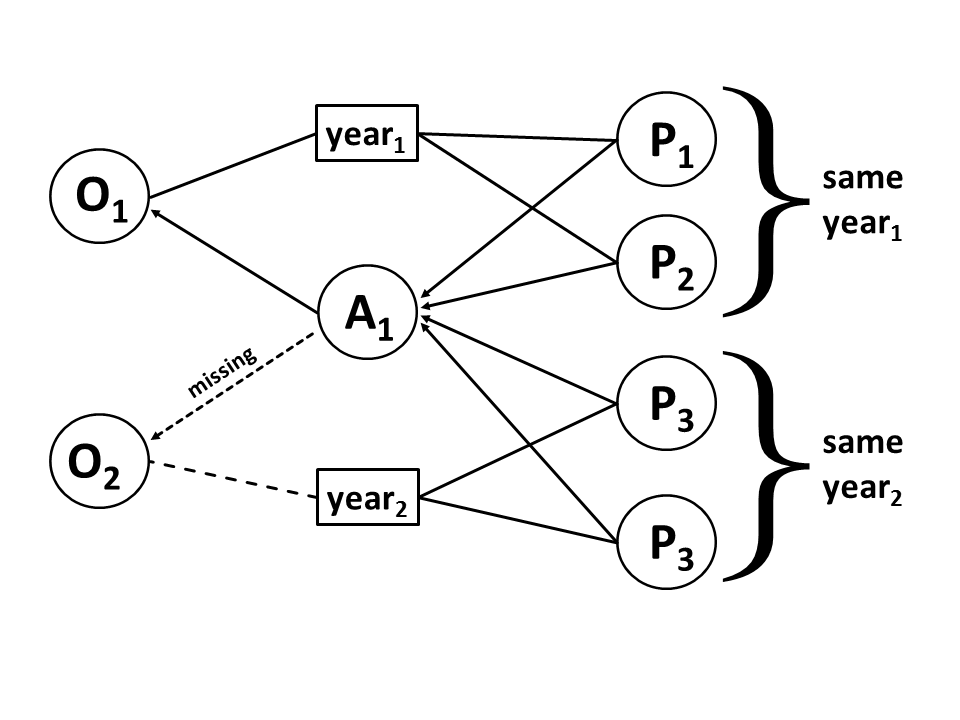
\includegraphics[width=0.25\textwidth, trim = 0mm 4mm 0mm 5mm, clip]{img/graph01.png}
    \caption{The part of the \textsc{msag} dataset illustrating missing organisation value issue. Markov Logic allows us to capture the following evidence: if two papers of the same author published in the same year, then they may published by the author of the same organisation. Nodes notation: A - denotes \textit{Author} entity; O - \textit{Organisation} and P - \textit{Paper} entities. Missing edges are marked as dashed lines.}
    \label{fig:msagmissing}
\end{figure}

\textbf{Evaluation metrics.} We evaluate the effectiveness of our data cleaning method, with a focus on two aspects: the accuracy and the performance of the method. To assess the accuracy of the data cleaning framework on relational data, we use \textit{Precision ($P$)}, \textit{Recall ($R$)} and \textit{F-measure ($F_1$)}. We acquire master data (referred to as \textit{"gold standard"}), which is clean and correct. We assess the efficiency of our method by running experiments on datasets of different sizes ranging from one thousand to one hundred thousand tuples each. We leverage a state-of-the-art inference engine for Markov logic called \textit{RockIt}~\cite{NoessnerNS13} and Gurobi solver version 5.6.3. All our experiments apply MAP inference for Statistical Relational Learning. We execute the experiments on a linux machine with an Intel 3.4GHz 4 Cores CPU and 16 GB of RAM.


%\subsection{Experimental Results} 
%\todo[inline]{For each experiment follow the structure: 
%1. Corresponding Contribution
%2. Experimental Setup (Dataset; Method)
%3. Results (Describe plots, measures etc.)
%4. Explanation (Why we have such results) and Relation to Contribution
%}



\subsection{Holistic Data Cleaning: Deduplication and Accuracy}
\label{subsec:exp1}
%%%%%%%%%%%
In this experiment we show that capturing the data issues interaction increases the overall accuracy in data cleaning. In particular, we study the connection between deduplication and improved data accuracy. We evaluate the accuracy of our method on different noise rates and different dataset sizes. We introduce noise by adding either typos or replacing values of attributes (active domain errors). We do not distinguish between these two kinds of errors. Table~\ref{tab:plots} shows the results of using Markov logic programs for data cleaning. The plots (a)-(c) illustrate the results for \textsc{hosp}, while plots (d)-(f) depict the results for \textsc{tpc-h}. %\note{DONT MAKE READERS THINK: Explain what readers see in these plots!!!} done.

In the first series of experiments, we fix the size for \textsc{hosp} and \textsc{tpc-h} to $90$K respectively $20$K tuples, while varying the noise rate from $2\%$ to $10\%$. The $x$-axis in Table~\ref{tab:plots} (a) and (d) represents the noise rate, the $y$-axis shows the corresponding $F_1$ measure values. First, we compare the results of separate executions of CDFs and MDs. After that we re-run the experiments with combined CFDs and MDs. When CFDs and MDs are modeled together in a single model for identifying dirty data, they are treated jointly and hence our method automatically picks the order of the data quality rules execution. The provided results in Table~\ref{tab:plots} (a) and (d) clearly demonstrate that jointly modeling CDFs and MDs improves the overall result because joint execution involves two processes simultaneously: matching (for values deduplication) and repair (for erroneous values). For this reason repairing supports matching and by identifying matches we are able to fix erroneous values.

In particular, the low $F_1$ score of MDs in Table~\ref{tab:plots} (a)-(b) and (d)-(e) results from low precision and high recall. However, By adding CFDs to MDs the overall $F_1$ score improves. The counterintuitive upward trend of the $F_1$ values while increasing noise in Table~\ref{tab:plots} (a) and (d) results from the \textit{Cutting Plane Inference} (CPI) \cite{riedel08improving} behavior. In all experiments, we use the CPI algorithm, which leverages optimization techniques such as Integer Linear Programming (ILP) \cite{riedel08improving, NoessnerNS13} by maximizing the objective function under set of constraints (every formula in MLN is being converted into a ILP constraint). CPI performs exact MAP inference and is guaranteed to converge in a finite number of steps \cite{riedel08improving}. For almost perfect data with less noise, the algorithm requires only a short runtime and converges fast by finding the approximately maximal objective score. This however results in detecting less data violations. Looking at the runtime in Table~\ref{tab:plots} (c) and (f), we recognise that with increasing noise the underlying solver calculates a solution until the maximum number of iterations is reached. For that reason, more data quality rule violations are encountered. 

In the second series of experiments, we fix the overall noise rate to 10\% on \textsc{hosp} (c.f.,~Table~\ref{tab:plots} (b)) and to 2\% on the synthetic \textsc{tpc-h} (c.f.,~Table~\ref{tab:plots} (e)). Afterwards we run three combinations of data cleaning rules on dataset sizes ranging from one thousand to one hundred thousand tuples each. In Table~\ref{tab:plots} (b) respective (e), the $x$-axis represents the data size and the $y$-axis shows the $F_1$-measure values. These two plots in (b) and (e) tell us that due to convergence guarantees of CPI our data cleaning method delivers robust results independently from the data size despite the increasing runtime of the algorithm (c.f.,~Table~\ref{tab:plots} (c) and (f)) by growing the dataset size. \anno{how do you see that? explain?}

Our results are in line with the observations made in \cite{Dallachiesa:2013:NCD:2463676.2465327}. There, the \textsc{nadeef} system demonstrates overall $F_1$-measure improvement. With a holistic treatment of FDs and MDs, \textsc{nadeef} achieves $0.8$ as $F_1$-measure. Due to using the identical data cleaning problem, the same evaluation methodology, as well as the same dataset \textsc{hosp}, we compare our results to theirs. Although their system demonstrates better performance for MD rules than ours, we get higher $F_1$-score values for the joint execution of the deduplication and accuracy rules: We achieve an overall performance $0.98$ and $0.99$ for \textsc{hosp} respectively \textsc{tpc-h} datasets and therefore report accuracy improvement by a factor of $1.2$ against this reference system.

We conclude from this experiment that the joint modeling and joint inference improves the accuracy achieved by running single data quality rules.

We also study the runtime of our method for different data sizes and noise rates. Table~\ref{tab:plots}~(c) for \textsc{hosp} and Table~\ref{tab:plots} (f) for \textsc{tpc-h} show the general trend for the runtime values ($y$-axis) for every data size ($x$-axis) setting. Each plot denotes different noise percentages. We see that the runtime on both, real-life and synthetic data, reveals an upward trend. Cleaning datasets with joint inference will take longer the larger the data is and the more noise it contains. In particular, for real-life \textsc{hosp} data of size $100K$ with increasing noise rate we observe runtime incrementing by factor $1.2$ for every noise setting. 
%\note{one plot shows linear increase, the other superlinear, mention and explain this!}. - hmm. for 10% and 8% for 100k on tpc-h sh** happens. and I do not know how to explain this without blaming rockit.
Additionaly, Table~\ref{tab:runtime} provides a detailed runtime values for different data sizes of \textsc{hosp} and \textsc{tpc-h} by fixing the noise to $4\%$. Here we observe that while data size increasing from twenty to $143$ thousands tuples, the average runtime growth rate is $1.9$. 
This is again a characteristic of the underlying MAP inference algorithm \textit{Cutting Plane Inference} \cite{riedel08improving}: Having less noise causes the algorithm converge faster, hence faster runtime values for data with less noise. %This experiment tells us that, while our method is robust against noise, but adding more noise leads to higher runtime. \anno{That is not a good finding, elaborate on the rate of runtime increase}


\subsection{Holistic Data Cleaning: Missing Value and Consistency Issues Interaction}
\label{subsec:exp2}
\pgfplotsset{small,  compat=1.5}
\begin{table*}[t]\footnotesize
\scriptsize
\centering
\begin{tabular}[t]{ll} %\hline
 
 \begin{tikzpicture}[baseline=0]
  %\begin{axis}[title=(a),
  %    xlabel=Recall,
  %    ylabel=$F_1$, ]
  %    \addplot+[only marks,mark=x] table[x=RECALL, y=F1] {data/msag-interpolated.tsv};
  %\end{axis}
    \begin{axis}[
      legend pos=outer north east,
      title=(a),
      xlabel=Recall,
      ylabel=F1, 
      legend entries={$1-2~missing~edges$,$3-4~missing~edges$,$more~than5$}, ]
         \addplot[ scatter,
                   only marks,
                   point meta=explicit symbolic,
                   scatter/classes={
                   a={mark=x,blue},%
                   b={mark=triangle,red},%
                   c={mark=o,draw=black}},] 
          table[x=RECALL, y=F1, meta=MARK] {data/msag-marked.tsv};
  \end{axis}
\end{tikzpicture}
&
 
 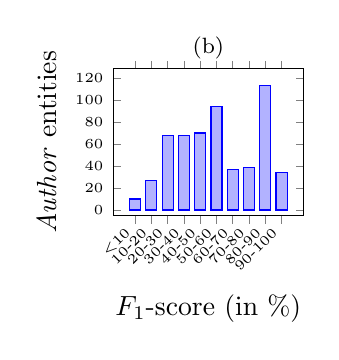
\begin{tikzpicture}[baseline=0]
        \begin{axis}[
        ybar,
        enlargelimits=0.15,
              %legend style={at={(0.5,-0.15)}, anchor=north,legend columns=-1},
        bar width=4,
        ylabel={\textit{Author} entities},
        xlabel={$F_1$-score (in \%)},
        title=(b),
        symbolic x coords={<10, 10-20, 20-30, 30-40, 40-50, 50-60, 60-70, 70-80, 80-90, 90-100},
        xtick=data,
        nodes near coords align={vertical},
        x tick label style={rotate=45,anchor=east},
        ]
        \addplot coordinates {(<10,10)
                              (10-20,27)
                              (20-30,68)
                              (30-40,68)
                              (40-50,70)
                              (50-60,94)
                              (60-70,37)
                              (70-80,39)
                              (80-90,113)
                              (90-100,34)};
        \end{axis}
      \end{tikzpicture}


 \\ %\hline
\end{tabular}
\caption{(a) \textsc{msag} cleaning: Recall and F1 values; (b) \textsc{msag} Experiments} 
\label{tab:msag}
\end{table*}

We extend the applicability of Markov logic to web data and provide initial results on cleaning the highly imperfect graph structured \textsc{MSAG} data set. We study the efficiency of data cleaning on web data by leveraging the connection between information completeness and data consistency. These two data issues interact with each other: missing values imputation helps to fix inconsistencies, and by correcting values missing entities can be identified. %In order to repair the attributes of an entity, they should not be missing and on the other hand, the data should be consistent for information completeness. \note{rewrite, sounds awkward}. -done.
In this experiment we partition our data and run inference for each author in isolation. We obtain a subgraph per \textit{Author}-entity with at least 10 \textit{Paper}-\textit{Author} edges. Next, we randomly select 600 \textit{Author}-entities. 

Table~\ref{tab:msag} (a) shows the accuracy achieved by our approach on the sample of \textsc{MSAG} dataset. We show the accuracy as relation between Recall ($x$-axis) and $F_1$-score ($y$-axis). We distinguish between three kinds of \textit{Author}-nodes (which are marked separately in Table~\ref{tab:msag} (a)): 
nodes with one or two missing \textit{Author}-\textit{Organisation} edges, nodes with three or four missing values for the \textit{Author} \textit{Organisation} connection, and finally nodes with more than 5 missing edges. Additionally, Table~\ref{tab:msag} (b) provides another perspective on this experiment by revealing the exact distribution of corrected \textit{Author}-entities ($x$-axis) by $F_1$-score ($y$-axis). The result shows the following: The method demonstrates overall $F_1$ score greater than $50\%$ and recall greater than $78\%$ for \textit{Author}-entities with one to two missing edges. Starting from three missing edges, we still achieve a recall ranging from $0.8$ to $1.0$, though the precision (and therefore $F_1$ score) drops. This happens because our approach selects more false positives with an increasing number of missing values. This experiment tells us that our method produces satisfying results on web data with very little noise only (e.g., missing values). In future work, extending data cleaning rules with domain specific information should be studied further in order to reduce the false positives rate. Because the \textsc{MSAG} dataset has only recently been published and related work in data cleaning systems provide results for cleaning relational data only, we are not able to compare ourselves to another system directly.

\subsection{Impact of Rule Execution Order}
\label{subsec:exp3}
Next, we study different orders of executing data cleaning rules, to show that specifying the optimal order of rules manually is hardly achievable~\cite{Dallachiesa:2013:NCD:2463676.2465327}. We investigate whether it is beneficial to leverage joint inference for simultaneous rule execution instead of manual specification of the optimal order of data cleaning rule execution. We verify the result in Figure~\ref{fig:orderexec} by investigating the $F_1$-score ($y$-axis) distribution of various data quality settings executed on varying noise rates ($x$-axis). We run our Markov Logic program on the attributes \textsl{state} and \textsl{zip} of the \textsc{hosp} dataset because they both participate in CFD and MD. Furthermore, we fix the dataset size at ninety thousands tuples with a noise rate varying from $2\%$ to $10\%$. Each experiment consists of three parts: First, we run the MD rules and then the CFDs, which gives us the overall worst accuracy. This results agree with the previous experiment about the joint modeling data cleaning rules (c.f.,~Table~\ref{tab:plots} (a) and Section \ref{subsec:exp1}). The MD rules perform poorer than CFDs. The overall $F_1$ score ranges between $0.01$ and $0.02$, which can be explained by really low precision and recall values due to error propagation from MDs to CFDs.  
In the second part of the experiment, we change the sequence of execution to running CFD rules before MD rules. This slightly improves the $F_1$ scores by increasing them from $0.1$ to $0.3$ for different noise values. We attribute this to the fact that CFDs initially detect more violations. However, analogous to the previous part, error propagation leads to the insufficient results. 

In the third and final part of the experiment, we perform the simultaneous execution of CFD and MD rules, meaning we modeled matching (for values deduplication) and repair (for erroneous values) processes together. Here we see a rapid increase of all accuracy values from $0.86$ for $2\%$ noise to $0.95$ on $10\%$ noise against the previously performed sequential execution of data cleaning rules. The growing trend of the $F_1$ scores has same explanation as results the experiment about holistic data cleaning (c.f.,~Table~\ref{tab:plots} (a) and Section \ref{subsec:exp1}) namely the functionality of the CPI algorithm. These results confirm our hypotheses that it is highly beneficial to execute multiple data cleaning rules simultaneously.  

The \textsc{nadeef} system~\cite{Dallachiesa:2013:NCD:2463676.2465327}, which also treats various types of rules holistically, ran an analogous experiment. Note that we report $F_1$-score improvements by factor $1.1$ on data with $10\%$ noise over the values reported by \textsc{nadeef}. 
%\note{rewrite sentence, tell readers factor of improvement as above}.
%\pgfplotsset{small,  compat=1.5}

\makeatletter
\let\percent\@percentchar
\makeatother
%\usetikzlibrary{patterns}

\begin{figure}
\centering
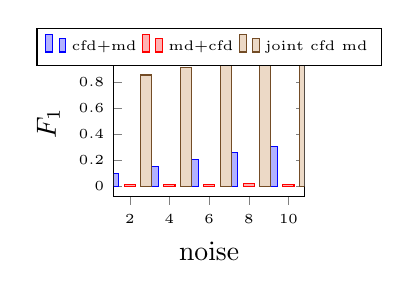
\begin{tikzpicture} 
\begin{axis}[
ybar,
enlargelimits=0.1,
legend style={at={(0.5,1.15)}, anchor=north, legend columns=-1},
bar width=4,
ylabel={$F_1$},
xlabel=noise,
symbolic x coords={{$2\percent$},{$4\percent$},{$6\percent$},{$8\percent$},{$10\percent$}},
xtick=data,
nodes near coords align={vertical},
]
\addplot coordinates {({$2\percent$}, 0.1) ({$4\percent$}, 0.1552) ({$6\percent$}, 0.2039) ({$8\percent$}, 0.2625) ({$10\percent$}, 0.3048)};
\addplot coordinates {({$2\percent$}, 0.0176) ({$4\percent$}, 0.0139) ({$6\percent$}, 0.0173) ({$8\percent$}, 0.0214) ({$10\percent$}, 0.016)};
\addplot coordinates {({$2\percent$}, 0.8566) ({$4\percent$}, 0.9114) ({$6\percent$}, 0.9403) ({$8\percent$}, 0.9512) ({$10\percent$}, 0.9569)};

%\addplot[pattern=north east lines] coordinates {({$2\percent$}, 0.1) ({$4\percent$}, 0.1552) ({$6\percent$}, 0.2039) ({$8\percent$}, 0.2625) ({$10\percent$}, 0.3048)};
%\addplot[pattern=dots] coordinates {({$2\percent$}, 0.0176) ({$4\percent$}, 0.0139) ({$6\percent$}, 0.0173) ({$8\percent$}, 0.0214) ({$10\percent$}, 0.016)};
%\addplot[pattern=horizontal lines] coordinates {({$2\percent$}, 0.8566) ({$4\percent$}, 0.9114) ({$6\percent$}, 0.9403) ({$8\percent$}, 0.9512) ({$10\percent$}, 0.9569)};

\legend{cfd+md,md+cfd,joint cfd md}

\end{axis}
\end{tikzpicture}
\caption{Execution order with Markov Logic} 
\label{fig:orderexec}
\end{figure}

%\subsection{Performance}



\subsection{Modeling Data Cleaning Rules}
\label{subsec:exp4}
%Big table containing all the rules and formulas:
\begin{table*}[t]\footnotesize
\scriptsize
\centering

\begin{tabular}{cll}
\textbf{\textit{Data Set}}               & \multicolumn{1}{c}{\textbf{\textit{Data Cleaning Rules}}}              & \multicolumn{1}{c}{\textbf{\textit{Markov Logic Formulae}}} \\ \hline
%hosp
\multirow{2}{*}{\textsc{hosp}}  & %hosp dq rules
                        \begin{tabular}[c]{@{}l@{}}
                        $\mathsf{cfd_1: \textsc{hosp}([\textsl{zip}] \rightarrow [\textsl{state, city}], t1=(\_ \parallel \_, \_))}$\\
                        $\mathsf{cfd_2: \textsc{hosp}([\textsl{phone}] \rightarrow [\textsl{addr, city}],t2=(\_ \parallel \_,\_,\_,\_))}$
                        \end{tabular}                   
                        & %hosp markov logic cfd
                        \begin{tabular}[c]{@{}l@{}}
                        $\mathsf{w_1: \textsl{zip}(id1, code)~\wedge~\textsl{zip}(id2, code)~\wedge \textsl{state}(id1, s1)~\wedge~\textsl{state}(id2, s2)~}$ \\
                        $\mathsf{~~~~~~~~\wedge!\textsl{state}(id1, s2)~\wedge~!\textsl{state}(id2, s1)~\Rightarrow \textsl{equal-state}(id1, id2)}$\\
                        %second cfd:
                        $\mathsf{w_2: \textsl{zip}(id1, code)~\wedge~\textsl{zip}(id2, code)~\wedge \textsl{city}(id1, c1)~\wedge~\textsl{city}(id2, c2)~}$ \\
                        $\mathsf{~~~~~~~~\wedge!\textsl{city}(id1, c2)~\wedge~!\textsl{city}(id2, c1)~\Rightarrow \textsl{equal-city}(id1, id2)}$
                        \end{tabular}                 \\ 
                       & %hosp md rule
                         \begin{tabular}[c]{@{}l@{}}
                        $\mathsf{md_1: \textsc{hosp}[\textsl{zip}]=\textsc{zipcode}[\textsl{zip}]\wedge \textsc{hosp}[\textsl{state}]\neq \textsc{zipcode}[\textsl{state}]}$\\
                        $\mathsf{~~~~~~~~~~~~~~\rightarrow\textsc{hosp}[\textsl{state}]\rightleftharpoons \textsc{zipcode}[\textsl{state}]} $
                        \end{tabular}                 
                       & %hosp markov logic md
                       \begin{tabular}[c]{@{}l@{}}
                        $ todo $
                       \end{tabular}                  
                       \\ \hline

%tpc-h
\multirow{2}{*}{\textsc{tpc-h}} & %tpc-h fds
                        \begin{tabular}[c]{@{}l@{}}
                        $\mathsf{cfd_1: \textsc{t}([\textsl{c\_custkey}] \rightarrow [\textsl{c\_name,c\_address}],t1=(\_ \parallel \_, \_))} $
                        \end{tabular}                   
                        &%tpc-h mlogic fds
                         \begin{tabular}[c]{@{}l@{}}
                        $ todo $
                        \end{tabular}                    
                         \\  
                       & %tpch md rules
                       \begin{tabular}[c]{@{}l@{}}
                        $\mathsf{md_1: \textsc{t}[\textsl{c\_address}]=\textsc{t}[\textsl{c\_address}] \rightarrow \textsc{t}[\textsl{c\_phone}]\rightleftharpoons \textsc{t}[\textsl{c\_phone}]}$\\ 
                        $\mathsf{md_2: \textsc{t}[\textsl{c\_name}]=\textsc{t}[\textsl{c\_name}] \rightarrow \textsc{t}[\textsl{c\_address}]\rightleftharpoons \textsc{t}[\textsl{c\_address}]} $

                        \end{tabular}                  
                       & %tpch md markov logic
                       \begin{tabular}[c]{@{}l@{}}
                        $ todo $
                        \end{tabular}                     
                       \\ \hline
%msag
\multirow{3}{*}{\textsc{msag}}  & % msag fd
                                \begin{tabular}[c]{@{}l@{}}
                                $\mathsf{cfd_1: \textsc{m}([\textsl{author\_id, year}] \rightarrow [\textsl{affiliation\_id}],t1=(\_,\_ \parallel \_))} $\\
                                $\mathsf{cfd_2: \textsc{m}([\textsl{affiliation\_id}] \rightarrow [\textsl{origin\_name}],t2=(\_ \parallel \_))} $
                                \end{tabular}                   
                                & %msag markov logic fd
                                \begin{tabular}[c]{@{}l@{}}
                                $todo $
                                \end{tabular}                   
                                \\  
                                & % msag extended fd
                                \begin{tabular}[c]{@{}l@{}}
                                 $\mathsf{eCfd_1: \textsc{m}([\textsl{author\_id, year}] \rightarrow [\textsl{affiliation\_id}],t1=(\_, diff(\_)\leq 2 \parallel \_))} $   
                                \end{tabular}             
                                & % msag markov logic 
                                \begin{tabular}[c]{@{}l@{}}
                                $ todo $
                                \end{tabular}  
                                \\
                                &%additional predicates for msag
                                %nothing here
                                & Equality axioms:
                                \begin{tabular}[c]{@{}l@{}}
                                $symmetry$\\
                                $transitivity$
                                \end{tabular}  

                                \\ \hline
\end{tabular}
\caption{\note{FINISH ME}Modeling data cleaning rules as Markov Logic programs.}
\label{tab:rulesformulas}
\end{table*}

%\note{This section would greatly benefit from a few concrete examples that show the benefits of modeling rules with markov logic!!! Furthermore, you need to explain how you measure usability!!!} - due to space limitations, I extracted all examples into a table. 
%\note{trying to elaborate the usability methodology from} \cite{Lewis2013UMUX, Finstad2010}
To asses usability of our method, we adopt research methodology from Usability Metric for User Experience (\textsc{umux-lite})~\cite{Lewis2013UMUX, Finstad2010} and discuss two items from \textsc{umux-lite} questionnaire: "Markov Logic capabilities meet requirements on data cleaning systems" and "Markov logic is easy to use". Being explained in former Sections \ref{sec:method}, \ref{subsec:exp1}, \ref{subsec:exp2} and \ref{subsec:exp3}, Markov logic indeed meet the main requirements on data cleaning systems such as \textit{holistic} data quality rules treatment \cite{Fan:2014:IRM:2628135.2567657, Dallachiesa:2013:NCD:2463676.2465327}, automation \cite{Stonebraker_datacuration} and heterogeneous rules incorporation \cite{chu2013holistic}. In the following we focus on the second item from \textsc{umux-lite} - "Markov logic is easy to use" - and provide our experience in how we modeled data cleaning rules by using Markov logic on all three datasets \textsc{hosp}, \textsc{tpc-h} and \textsc{msag}. %Table \ref{tab:rulesformulas}

\textbf{\textsc{hosp} Quality Rules}. In our data cleaning method for the \textsc{hosp} data, we use 6 manually designed CDFs and one MD, which result in 15 normalized CFDs. One MD rule is transformed into 2 formulas. All data cleaning rules are positive. Finally, all interleaved rules are translated into 21 Markov logic formulas. In the Table \ref{tab:rulesformulas}, we provide an example of these data quality rules, which are defined on pairs of tuples. The MD rule is specified on a two relations. Markov logic predicates used for data quality formulas are shown in Table~\ref{tab:predicates}. After transforming the 100k \textsc{hosp} tuples into Markov logic grounded atoms, the resulting data comprises 1.3M evidence atoms, which will be used for inference. We empirically observe that extending the data quality rules set for additional conditions, which makes consideration of similar tuples unnecessary and reduces the search space and therefore converges much faster than \textit{"pure"} model. This means that each first order logic formula, which represent the RHS of the normalized data quality rule $\mathsf{\textsl{attr}(id1, v1)~\wedge~\textsl{attr}(id2, v2)}$ becomes an inverse part $\mathsf{!\textsl{attr}(id1, v2)~\wedge~!\textsl{attr}(id2, v1)}$. This additional part denotes that we consider only tuples with different values. Here the normalized CFD rules are being compiled as demonstrated in the Table \ref{tab:rulesformulas}. 
%\note{What has this whole paragraph to do with usability? How did you measure it? What is the purpose of this discussion?}

\textbf{\textsc{tpc-h} Quality Rules}. We write 9 CFDs and 3 MDs for this dataset. One example of the rules is a CFD that states if two tuples agree on \textsl{c\_custkey}, then they should agree on \textsl{c\_name} and \textsl{c\_address} attributes. MDs are designed on the same schema \textsc{tpc-h} \textsl{(T, T)}. These MDs state that for any pair of tuples $(t_1,t_2)$ if the LHS is similar, then the attribute values on the RHS should be identified. In the Table \ref{tab:rulesformulas} we provide an except of the data quality rules we created for \textsc{tpc-h}. Markov logic predicates used for data quality rules are shown in Table~\ref{tab:predicates}. After transforming the 100k \textsc{tpc-h} tuples into Markov logic grounded atoms, the resulting data comprises 1 Mio evidence atoms, which are then used for inference. 
%\note{Again: What has this whole paragraph to do with usability? How did you measure it? What is the purpose of this discussion?}

\textbf{\textsc{msag} Quality Rules}. Due to the graph nature of the \textsc{msag} data (c.f.,~Figure \ref{fig:msagmissing}) we develop data quality rules, which are based on CFDs, \textit{extended} CFDs \cite{Chen2009extended} and equality axioms, such as \textit{symmetry} and \textit{transitivity}. For the \textit{Paper}-\textit{Author}-\textit{Organisation} subgraph we define two CFDs, one extended CFD and 8 additional rules that comprises equality axioms for hidden predicates. Considering the semantical meaning of the data, we profit from the ability to add supporting knowledge into data cleaning process. For example, having the CFD $\mathsf{\textsc{m}([\textsl{author\_id, year}] \rightarrow [\textsl{affiliation\_id}],t1=(\_,\_ \parallel \_))} $  allows us to capture all missing affiliation by the same author, which published in the same year. In real life we know that in academia an average contract lasts around 2-3 years. Therefore by incorporating this knowledge in form of a predicate $\mathsf{\textsl{inRange}(year, year)}$, we will extend our search range. Additionally, by combining with equality axioms, we enable capturing more missing values. For example, the hard rule $\mathsf{\textsl{equal-Affiliation}(id_1, id_2) ~\wedge~ \textsl{equal-Affiliation}(id_2, id_3) \Rightarrow  \textsl{equal-Affiliation}(id_1, id_3)}$ denotes transitive relationship between three different entities \textit{Organisation}. In total, Markov Logic program consists then from 21 lines of code and an except can be viewed in the Table \ref{tab:rulesformulas}. 
%\note{Again: What has this whole paragraph to do with usability? How did you measure it? What is the purpose of this discussion?}

This part of our experimental study demonstrates that the expressiveness of Markov Logic affords us to model data cleaning rules. While existing data cleaning systems \cite{Dallachiesa:2013:NCD:2463676.2465327} are also concerned about the generality of the data cleaning rules, we can define Markov Logic data cleaning rules in expressive first-order logic manner without the need to implement any code. Furthermore, Markov Logic is data format independent, which facilitates data cleaning on different data formats as provided on relational and graph data formats. 

\subsection{Summary}
%\note{Add references to the individual chapters when you summarize! Does this summary cover all experiments?}

The results of our experimental study indicate that multiple types of data cleaning rules should be considered \textit{holistically} (Section \ref{subsec:exp1} and \ref{subsec:exp2}), which confirms previous research \cite{Dallachiesa:2013:NCD:2463676.2465327, Fan:2014:IRM:2628135.2567657, Fan:2011:IRM:1989323.1989373}. Adding domain or structural knowledge about data into the Markov logic program improves overall data cleaning. Furthermore, by using joint inference we are able to achieve very good results without defining the order of the data cleaning rules execution. We find that joint modeling of data quality rules results in higher accuracy of data correction (Section \ref{subsec:exp3}). By using the probabilistic-logical framework Markov logic we benefit from its flexibility in constraints definition and joint inference over different data repair and match rules. The direct translation of data cleaning rules into first-order logic (and therefore Markov Logic formulas) simplifies the process of writing data cleaning routines (Section \ref{subsec:exp4}). 

%%%%%%%%%%%%%%%%%%%%%%%%%%%%%%%%%%%%%%%%%%%%%%%%%%%%%%%%%%%%%%%%%%%%%%%%
% Related Work
%%%%%%%%%%%%%%%%%%%%%%%%%%%%%%%%%%%%%%%%%%%%%%%%%%%%%%%%%%%%%%%%%%%%%%%%
\section{Related Work}
\label{sec:related}

Our research builds on previous work from two areas: 
\begin{inparaenum}[\itshape 1\upshape)]
\item Data quality management and
\item Statistical relational learning, namely probabilistic-logical languages.
\end{inparaenum}

\textbf{Data Quality Management}: A rich theoretical and practical investigation into data cleaning was presented in~\cite{Fan:2014:IRM:2628135.2567657} and \cite{fellegi1976systematic}. Fan W. et al.~\cite{Fan:2011:IRM:1989323.1989373} first proposed to unify the record matching and data repairing processes. They also proved that this unification greatly contributes to the improvement of the data quality. Based on this fundamental research, we propose to use probabilistic-logical frameworks to model the interaction of data quality rules and show that Markov logic enables us to simultaneously use MDs and CFDs. Holistic data cleaning methods based on integrity constraints and denial constraints with ad-hoc predicates have also been studied in \cite{chu2013holistic}. This approach considers the generalization of integrity constraints by translating them into denial constraints. However, denial constraints cannot express inclusion dependencies, hence in our work, we use the clausal form of the first-order predicate logic to express all kinds of integrity constraints. A generalization of dependencies was proposed by the Llunatic system in \cite{llunaticVDLB2013b}. They introduce a new language based on equality generated dependencies to standardize the way in which to express intra- and inter-dependencies. A clustering-based declarative approach for deduplication based on data constraints has been suggested in the Dedupalog language in \cite{Arasu:2009:LDC:1546683.1547340}.

The \textsc{Nadeeff} system from \cite{Dallachiesa:2013:NCD:2463676.2465327} is the system closest to ours with regard to the coverage of requirements for data cleaning systems. Analogous to our system, they treat data quality rules holistically. In contrast to \textsc{Nadeeff}, 
\begin{inparaenum}[\itshape 1\upshape)]
	\item we use first-order logic to define all the kinds of data quality rules and, therefore do not need black-boxes in the form of user-defined functions. Furthermore, we claim a higher usability of the system through ability to declaratively formulate rules;
	\item we perform data cleaning as an inference process on Markov networks. The inference is fully hidden from the user, which achieves a substantial complexity reduction.
\end{inparaenum}  

Relevant work in statistical inference and data cleaning has been conducted by Mayfield and his team in~\cite{Mayfield:2010:EDA:1807167.1807178}. Their system \textsc{Eracer} has been designed to perform missing values imputation. In our work, we also use statistical inference to predict missing values, repair data, and detect duplicate entries. We apply MAP inference to infer the types of errors and their sources. We also assume that the data quality rules based on FDs, CFDs, and MDs are already defined. Song and Chen, as well as Fan W. et al. present profiling algorithms to discover CFDs and MDs automatically~\cite{song2009discovering,Fan:2011:DCF:1978258.1978514}. Applying machine learning for entity deduplication has been demonstrated in \cite{guo2010record}. The work in \cite{beskales2010probclean} uses a probabilistic model for duplicate detection with uncertain outcomes. Throughout our work we use SRL, which is an extension of machine learning with respect to existing relations in the data.

The most recent work in data curation that subsumes data cleaning is the Data Timer System~\cite{Stonebraker_datacuration}. The researchers present an end-to-end system that performs massive data curation and data deduplication by combining two elements: machine learning and expert (human) feedback. In our work, we emphasize the joint execution of data cleaning rules, which are declared as \textit{soft} or \textit{hard}. Furthermore, we do not require human input to achieve high accuracy results, instead, we fully rely on the MAP-inference results to predict errors. Using machine learning and likelihood methods for cleaning noisy databases by predicting possible data updates has been introduced in \textsc{SCARE} system \cite{Yakout:2013:DSU:2463676.2463706}. In contrast to \textsc{SCARE}, our solution is capable of modeling and predicting not only missing values imputation and data consistency but also data deduplication. 

\textbf{Statistical Relational Learning}: An advantage of probabilistic modeling for data quality has been investigated in~\cite{doi:10.1080/01621459.1972.10481323} and~\cite{chen2011usher}. Markov logic as a formalism for joint inference has been successfully used in a number of tasks, including natural language processing \cite{che2010jointly, riedel08collective, meza09jointly}, ontology alignment, data integration~\cite{niepert2011probabilistic} and co-reference resolution~\cite{poon2008joint,singla2006entity}. These research results demonstrate the advantage of joint modeling vs. pipeline execution. We are the first to apply this formalism to data cleaning and to show the benefits of a joint data cleaning approach that uses MLNs as a framework for interacting data quality rules. 



%%%%%%%%%%%%%%%%%%%%%%%%%%%%%%%%%%%%%%%%%%%%%%%%%%%%%%%%%%%%%%%%%%%%%%%%
% Conclusion
%%%%%%%%%%%%%%%%%%%%%%%%%%%%%%%%%%%%%%%%%%%%%%%%%%%%%%%%%%%%%%%%%%%%%%%%
\section{Conclusion and Future Work}
\label{sec:conclusion}
In this paper, we presented a declarative data-cleaning approach based on statistical relational learning and probabilistic inference. Generally, data quality rules represent relationships between attributes in the database schema and these rules are mainly based on functional dependencies on top of a database schema. We demonstrated how such functional dependencies, expressed as first-order logic formulas, can be translated into probabilistic logical languages, allowing us to reason over inconsistencies or duplicates in a probabilistic way. Our approach allows the usage of probabilistic joint inference over interleaved data cleaning rules to improve data quality. By using a declarative probabilistic-logical formalism such as Markov logic, we are potentially able to incorporate more semantic constraints (latent semantic factors) and, therefore, extend traditional data quality rules. We are currently extending the algorithm to massive data set settings and preliminary results are encouraging. With regards to experimenting with modeling additional semantic constraints, larger and more heterogeneous data sets, present and future research will focus on the improving data quality for distributed data. The results that we have presented in paper indicate that taking a holistic view on data cleaning and that modeling this intuition within a Markov logic framework is a feasible and effective means to create data cleaning systems. 


\bibliographystyle{abbrv}
\bibliography{sigproc} 
\balancecolumns

\end{document}
